\documentclass[a4paper,12pt]{jsarticle}
\usepackage[dvipdfmx]{graphicx}
\usepackage{here}
\usepackage{url}
\usepackage{lmodern}
\usepackage{textcomp}
\usepackage{latexsym}
\usepackage[fleqn]{amsmath}
\usepackage{float}
% 下の3行のコメントを外すと原稿チェックのための行番号がでる
%\usepackage{lineno}
%\linenumbers
%\modulolinenumbers[5] % 5行ごとに行番号を出す 閲覧用

\begin{document}

%%-----------------------------------------------------------------------
%% 表紙
%%-----------------------------------------------------------------------
\begin{titlepage}
\begin{center}
\fontsize{14pt}{0pt}\selectfont
\par
千葉工業大学\\
修士学位論文

\vspace{3cm}

\fontsize{14pt}{3pt}\selectfont
\par
%% タイトル
\Huge 時空間永続証明のための\\
\Huge ブロックチェーン履歴交差法の検討\\

\vspace{7cm}

\fontsize{14pt}{1cm}\selectfont
\par
所属専攻:電気電子情報工学専攻
\vspace{0.25cm}

\fontsize{14pt}{0pt}\selectfont
\begin{tabular}{lll}
%% 氏名および学生番号
学籍番号・氏名:1972042 & 柳原 貴明 \\
\end{tabular}

\vspace{1cm}

\par
指導教員:藤原 明広 准教授

\vspace{1cm}

\par
%% 提出日
提出日 令和3年 3月dd日
\end{center}
\end{titlepage}

\normalsize
\pagenumbering{roman}


%%----------------------------------------------------------------------
%% 概要
%%----------------------------------------------------------------------
\section*{概要}
最後に書く


\newpage
%%----------------------------------------------------------------------
%% 目次
%%----------------------------------------------------------------------
\tableofcontents
\newpage

%%----------------------------------------------------------------------
%% 本文
%%----------------------------------------------------------------------
\pagenumbering{arabic}

%%----------------------------------------------------------------------
\section{序論}
%%----------------------------------------------------------------------
近年,クラウドコンピューティングおけるデータサーバーの仮想化を代表されるような
ストレージやネットワーク,アプリケーションなどの様々な機能が仮想化技術によって提供されている.
利用者は,メンテナンスフリーや維持費の安さなど利点は多くあり普及が加速しているが
データサーバーを管理する大きな力を持った企業・組織に依存することになる.

Bitcoinを代表とする(パブリックな) ブロックチェーンは,世界中に散在するコアノード同士で,
取引データやブロックを転送するため頻繁に共有し合っている.
地理的に近いコアノード同士では通信遅延時間の影響は少ないが,
遠距離のノードにブロックを転送する場合,数十秒〜数分の通信遅延が起きる.

現状では,Proof of Work( PoW )によるブロック生成時間を十分遅くする必要がある
この理由によりビットコインではブロック生成時間が10分になるように制御されている.
従って遅延時間により,単位時間に処理可能な取引量が少なくなる.
これは「スケーラビリティ問題」として知られている. 
この問題を解決する方法の一つとして,地理的に近いコアノード同士でドメインを自律的に形成し,
ドメイン毎に独自のブロックチェーンを管理する方法が提案されている \cite{fujihara1}\cite{fujihara2}.
しかし,各ドメインに存在するコアノードの数が減少するため,
ブロックチェーンの非中央集権性と改ざん耐性が低下する問題があった.
本章では,本研究の背景として現状の動向と先行研究の問題点を挙げ,本研究目的を述べる.


\subsection{背景}
\subsection*{Bitcoin: A Peer-to-Peer Electronic Cash Systemの誕生}
近年,クラウドコンピューティングおけるデータサーバーの仮想化を代表されるような
ストレージやネットワーク,アプリケーションなどの様々な機能が仮想化技術によって提供されている.
利用者は,メンテナンスフリーや維持費の安さなど利点は多くあり普及が加速しているが
データサーバーを管理する大きな力を持った企業・組織に依存することになる.
金融界におけるBitcoin誕生以前は,インターネットバンキング等の電子取引は,ほぼ例外なく,
信用することのできる第三者機関に金融機関に依存しているのが現状であった.
Bitcoinは,信用ではなく暗号化された証明に基づく電子取引システムであり,
これにより希望する二者が信用できる第三者機関を介さずに直接取引ができる.
従って,金融界の中央集権性を否定している.
非中央集権性を可能にする技術がブロックチェーンである.
ブロックチェーンは,金融界だけでなく様々な業界での応用が期待されている.

\subsection*{Bitcoinブロックチェーンのスケーラビリティ問題}
Bitcoinを代表とする(パブリックな) ブロックチェーンは,世界中に散在するコアノード同士で,
取引データやブロックを転送するため頻繁に共有し合っている.
図 \ref{fig:bitnodes} に2020年11月17日現在の全世界のBitcoinコアノードの分布を示す.

\begin{figure}[H]%挿入図
  \begin{center}
    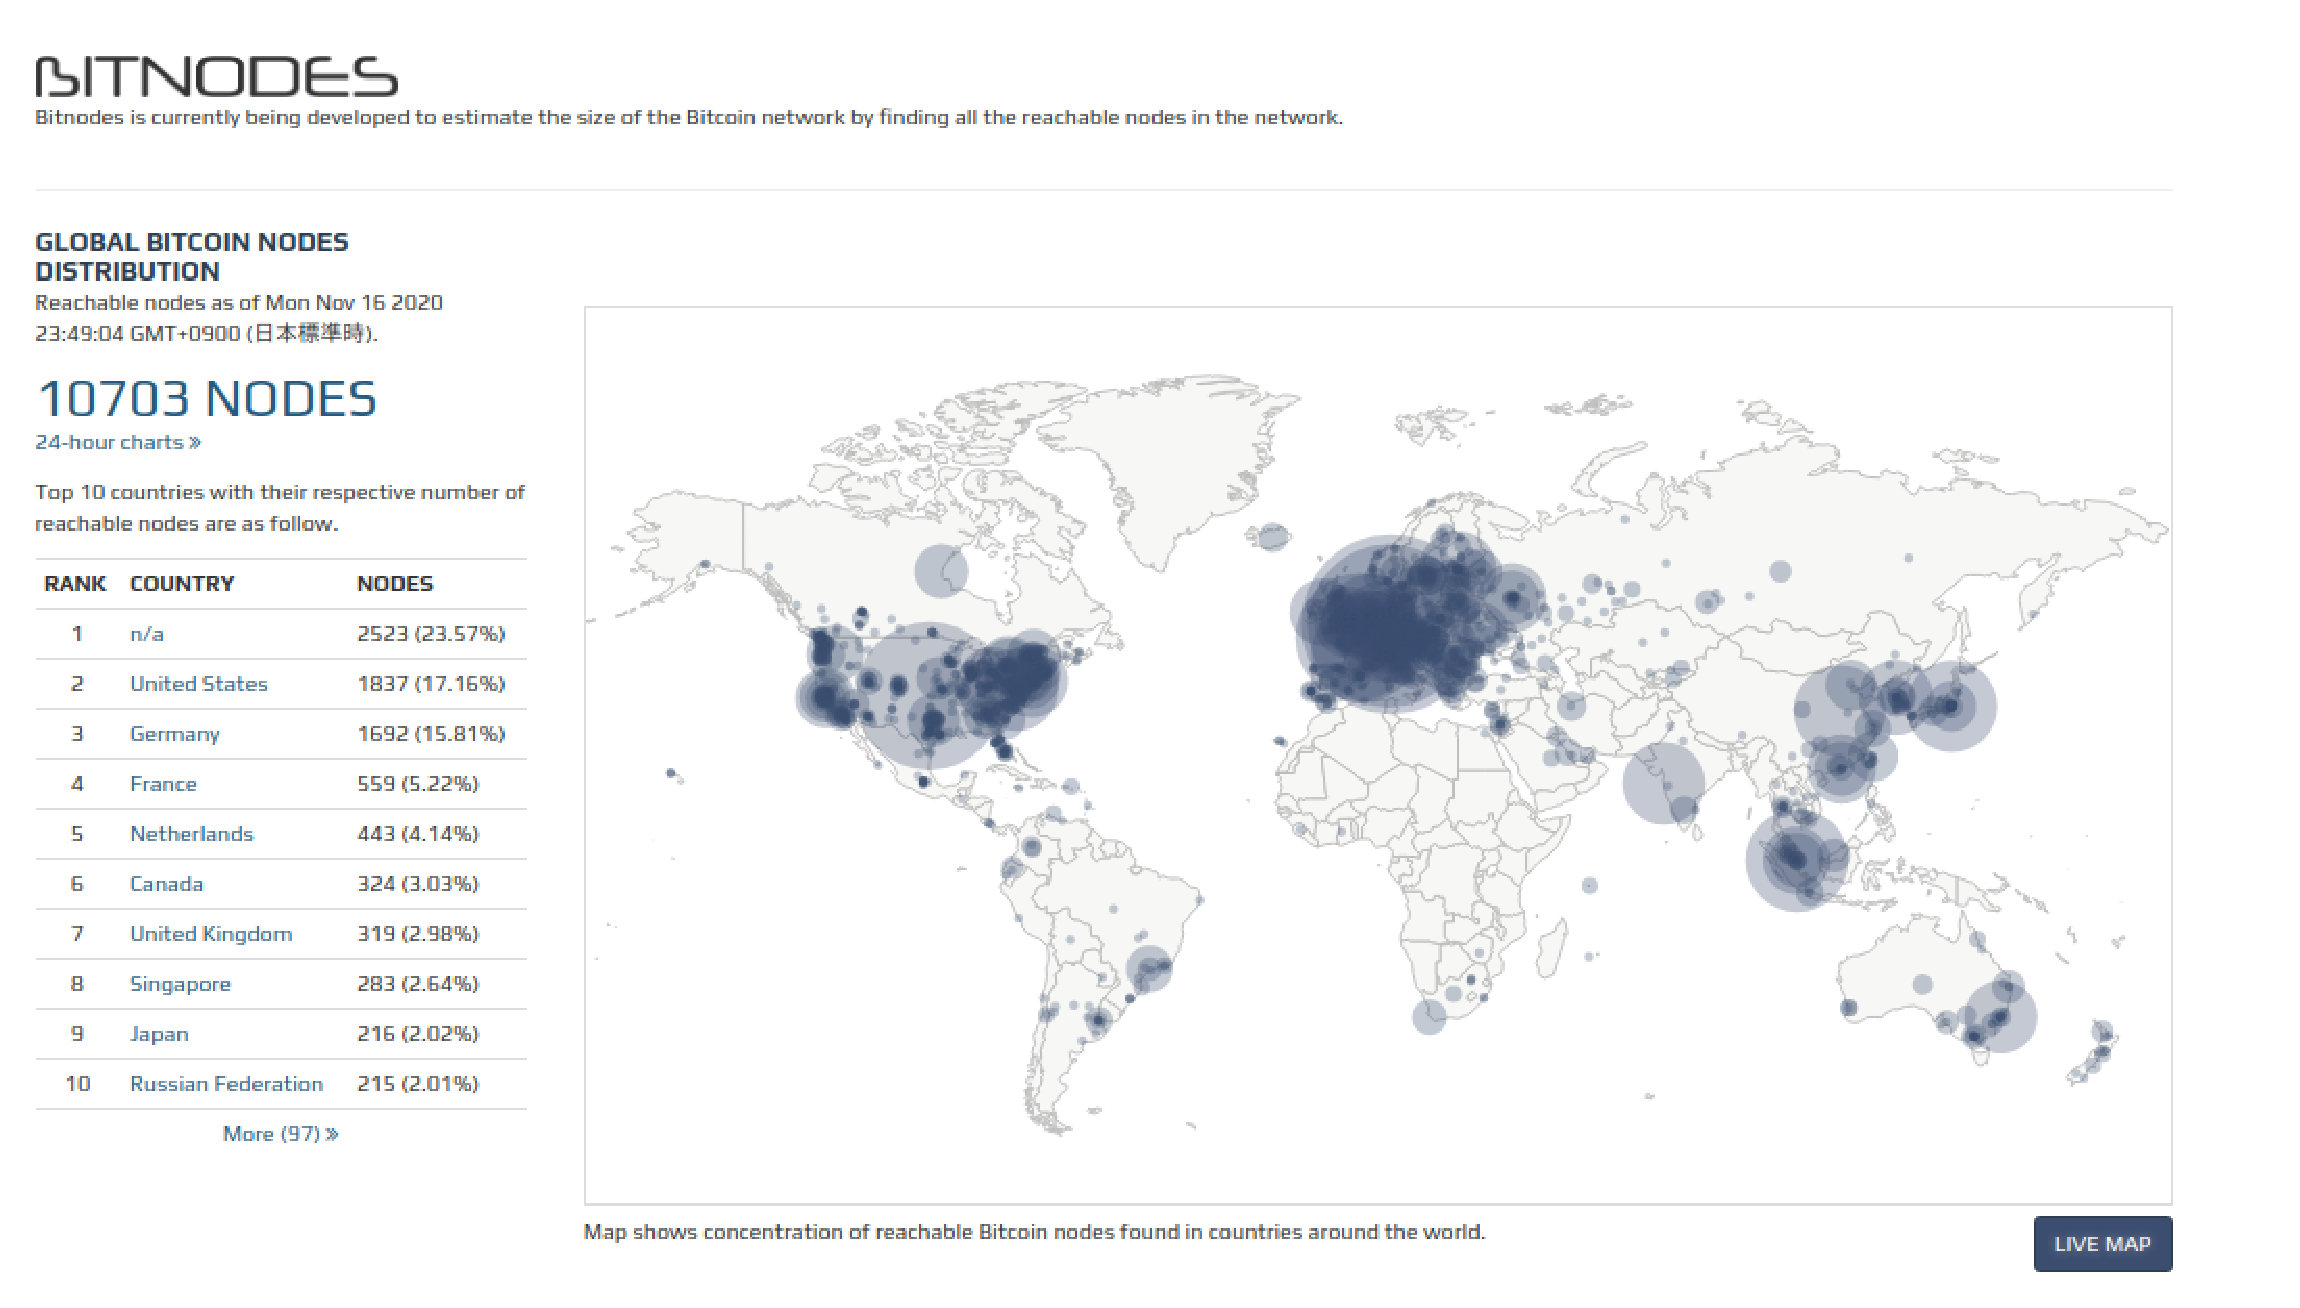
\includegraphics[width=130mm]{pht/bitnodes1117.eps}
  \end{center}
  \caption{2020年11月17日現在の全世界のBitcoinコアノード分布}
  \label{fig:bitnodes}
\end{figure}

地理的に近いコアノード同士では通信遅延時間の影響は少ないが,
遠距離のノードにブロックを転送する場合,数十秒〜数分の通信遅延が起きることが知られている.
この通信遅延により,Proof of Work( PoW )によるブロック生成時間を十分遅くする必要がある
従って,ビットコインではブロック生成時間が10分になるように制御されている.
この遅延時間により,単位時間に処理可能な取引量が少なくなる.
これは「スケーラビリティ問題」として知られている. 

\subsection*{スケーラビリティの問題へのアプローチ}
ブロックチェーンのスケーラビリティ問題に対するほとんどの解決策は,
コンセンサスプロトコルの改善,ブロックサイズの縮小,ネットワークスケーリングのいずれかになる.
ブロックサイズのサイズの縮小は,Off-chainの考え方であり,情報量を必要最低限に削減し,
通信遅延等のスケーラビリティ問題への解決を目指す提案が行われているが,スケーラビリティ問題の本質的な改善にはならない.
本研究では,従来のブロックチェーンの情報量を削減しない(On-chain)方法でのスケーラビリティ問題を改善を行う.

\subsection{本研究の目的}
先行研究では,ドメイン分割を行い通信距離による通信遅延を削減し,
地理的に近いコアノード同士でドメインを形成し,ドメイン毎に独自のブロックチェーンを管理する方法が提案されている.\cite{fujihara1}\cite{fujihara2}.
しかし,単にドメイン分割を行うと各ドメインのブロックチェーンに関わるコアノードの数が減少する.
これにより,ブロックチェーンの特性である非中央集権性と改ざん耐性が低下する問題がある.
そこで本研究では,ブロックチェーンの状態を定期的に共有し,各ドメインのブロックチェーンに
互いの署名 (ヒステリシス署名) を書き込み合う履歴交差法を提案し,先行研究で挙げれる
非中央集権性低下と改ざん耐性の低下してしまう問題を改善することを目的としている.

\newpage
%%----------------------------------------------------------------------
%\section{関連技術動向と関連研究}
%%----------------------------------------------------------------------
\section{関連研究}
\subsection{BBc-1}
BBc-1\cite{saito}は,プライベートな取引データを履歴交差により改ざん耐性を持たせて
保存する (ブロックチェーンではない) 分散台帳技術である.
ノードの実装も行われており,その有効性が実験的にも確認されている.
BBc-1では,取引データにヒステリシス署名を追加する.
ヒステリシス署名を取引データに付けて,ドメイン間でデータを共有することで改ざん耐性を高めている.
また,PoWによる改ざん耐性の向上を行わない為,エネルギーコストは低く済む特徴がある.
しかし,改ざん耐性がどの程度向上したかを理論的に評価しにくいことも知られている.

\subsection{bloXroute}
bloXroute \cite{bloX} では,P2Pネットワーク上で取引データやブロックの共有速度を早める為に,
構造化されたネットワークを(Layer0と呼んでいる)上位ネットワークに構築する提案を行っている.
PlasmaやShardingのようなプロトコルがレイヤー2のソリューションとみなされるなら,
bloxrouteはレイヤー0のスケーラビリティソリューションとして分類される.
これらのレイヤ2スケーラビリティ・プロトコルの多くは,
現在の世代のブロックチェーン技術で広く採用されるようになる可能性が高いが,
空間の細分化にも貢献している.
bloxRouteはそれらの従来のモデルを無視し,あらゆるブロックチェーンの下で動作するソリューションを提案している.

bloxRoute は,レイヤー0のプロトコルで,ブロックチェーンの全体的なアーキテクチャに影響を与えることなく,オンチェーン全体で数桁の増加を可能にします.
bloXroute BDNは,ブロックチェーンの下で分散型ルーターとして機能することで,高いレベルのスケーラビリティを実現している.

bloXrouteは,スケーラビリティ問題に対するアプローチは,既存のブロックチェーンの基礎となるプロトコルを崩すことなく,
ブロックチェーンネットワークにおけるスケーラビリティの問題を解決する独自のアプローチを提案している.
bloXrouteは,ブロックチェーンに関しては対立することが多い3つの原則,すなわちスケーラビリティ,中立性,適応性を兼ね備えている.
このプラットフォームは,あらゆるブロックチェーンに組み込むことができる効果的な
ブロードキャスト・プリミティブを実装することで,スケーラビリティを提供している.
暗号化されたブロックをサポートすることで中立性を実現し,ピアリレーでブロックの出所を不明瞭にすることで中立性を実現している.
最後に,ユーザがゲートウェイを介してネットワークを系統的に直接かつ積極的に調査できるようにすることで,監査可能性を実現している.

\subsection{PoWaP(Poof of Work at Proximity for a crowdesnsing system)}
PoWaPとは地理的に近いノード同士が空間領域(ドメイン)を構成して蜜になるネットワークを構成することで,
ドメイン毎に独自のブロックチェーンを管理するネットワークシステム\cite{DomainSplit} に概要図を示す.
ドメインに分割して制御することで,ブロックの生成する時間が短縮可能である.
また,利用者は近くのノードに近距離無線通信でアクセスして取引等の情報を送ることで,ドメイン(地域)に
特化した情報をブロックチェーンに保持させることも可能になる.

\subsection{Atomic Swap}

Atomic Swapは異なるチェーン間で相手を信用することなく,アトミックにコインを交換するのに使用されるプロトコルである.一般的なプロトコルとしてはHTLCが利用される.

アリスがBitcoinを持ち,ボブがLitecoinを持っている状態でアリスとボブはそれぞれBitcoinとLitecoinを交換したい場合,
以下のような手順で相手を信用することなく各チェーンのコインをアトミックに交換できる.

\begin{enumerate}
  \item アリスはシークレットAをランダムに選択し,そのハッシュ値H(A)をボブに伝える.
  \item アリスは自分のBitcoinを以下のいずれかの条件でアンロック可能なスクリプト宛に送金するトランザクションを作成しBitcoinネットワークにブロードキャストする.
%
  \begin{itemize}
    \item H(A)のプリイメージを提供すればボブの鍵でアンロック可能.
    \item 2日後アリスの鍵でアンロック可能.
  \end{itemize} 
  \item ボブは自分のLitecoinを以下のいずれかの条件でアンロック可能なスクリプト宛に送金するトランザクションを作成しLitecoinネットワークにブロードキャストする.
%
  \begin{itemize}
    \item H(A)のプリイメージを提供すればアリスの鍵でアンロック可能.
    \item 1日後ボブの鍵でアンロック可能.
  \end{itemize}
%
  \item アリスはシークレットAを使って3のボブのLitecoinを入手するトランザクションを作成しLitecoinネットワークにブロードキャストする.
  \item ボブはLitecoinのブロックチェーン上で4のトランザクションを確認することでシークレットAの値がわかる.
  \item ボブはシークレットAの値を使って2のアリスのBitcoinを入手するトランザクションを作成しBitcoinネットワークにブロードキャストする.
\end{enumerate}

同様に本研究におけるドメイン間で分割を行った異なるブロックチェーン間の取引データも,Atomic Swapで用いることで情報のやり取りができる.

\subsection{Raft Consensus Algorithm}\cite{Raft Consensus Algorithm}
\label{Raft}
複数のノード間で合意を得る必要がある.
分散システムで合意するを得る手段にRaftがある
RaftはPaxosど同等の性能を持ちながらPaxosよりも格段の理解のしやすさを提供する分散合意プロトコルである.
%Raftのアーキテクチャ概要を図1に示す.要追加
Raftを実行するノードには, LEADER,CANDIDATE,FOLLOWERという$3$種類の状態がる.LEADERはクラスタ内に1台しか存在しない.
クライアントは,LEADERノードとインタラクションする.クライアントはLEADERにアクセスしてきた場合はLEADERにリダイレクトされる.
FOLLOWERのノードはLEADERノードに従う.LEADERノードはクライアントノードから更新要求を受信すると,ログレコードを作成する.そしてLEADERノードはログレコードをストレージに保存した後,ログレコードをログレコードをFOLLOWERノードへ転送する.
FOLLOWERノードは受信したログレコードをストレージに保存すると,ACKをLEADERへ送信するLEADERを含め,Raftクラスタの過半数が命令を受け取ったことをLEADERが確認した後,クライアントにCOMMITを通知する.
最終的には,すべてのノードが同じ命令を同じ順番で実行するため,すべてのノードでデータが複製される.
即ちRaftは複製化状態機械に基づいて設計されている.一般に利活用されている複製化状態機械に例として,Chubby,ZooKeeperなどが挙げられる.
LEADERノードが故障したり,LEADERノードの故障したり,LEADERノードのネットワークコネクションが切断されると,Raftクラスタ内にLEADERが存在しなくなる.
このような場合,FOLLOWERノードは状態をCANDIDATEへと変更する.
クラスタ内のノードは各CANDIDATEへの投票を行い,新たなLEADERを選出する.
この選出にはクラスタを構成するノードの数の過半数の選任が必要である.
過半数を得たノードが存在しなければ,LAEDER選出作業を再実行する.

%--------------------------------------------
\newpage
%--------------------------------------------
\section{関連技術動向}
ソフトウェアシステムの構造(アーキテクチャ)には大きく「集中システム」と「分散システム」の2つがある.
図のように集中システムは1つの中心があり,そこに他のコンピュータが接続する形になっており,

\begin{figure}[h]%挿入図
  \begin{minipage}{0.5\columnwidth}
    \centering
    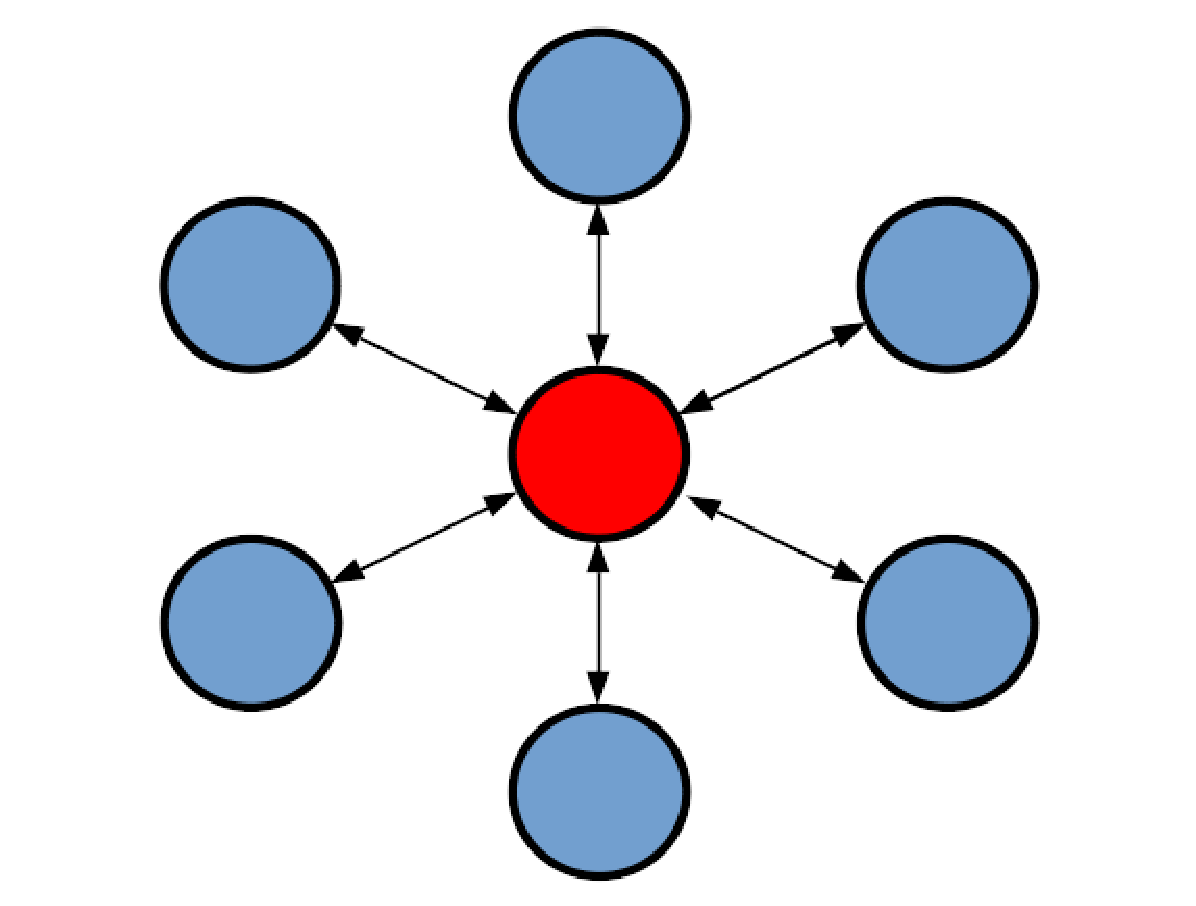
\includegraphics[width=50mm]{pht/CentralizedSystem.eps}
    \caption{集中システム}
    \label{fig:CentralizedSystem}
  \end{minipage}
  \begin{minipage}{0.5\columnwidth}
    \centering
    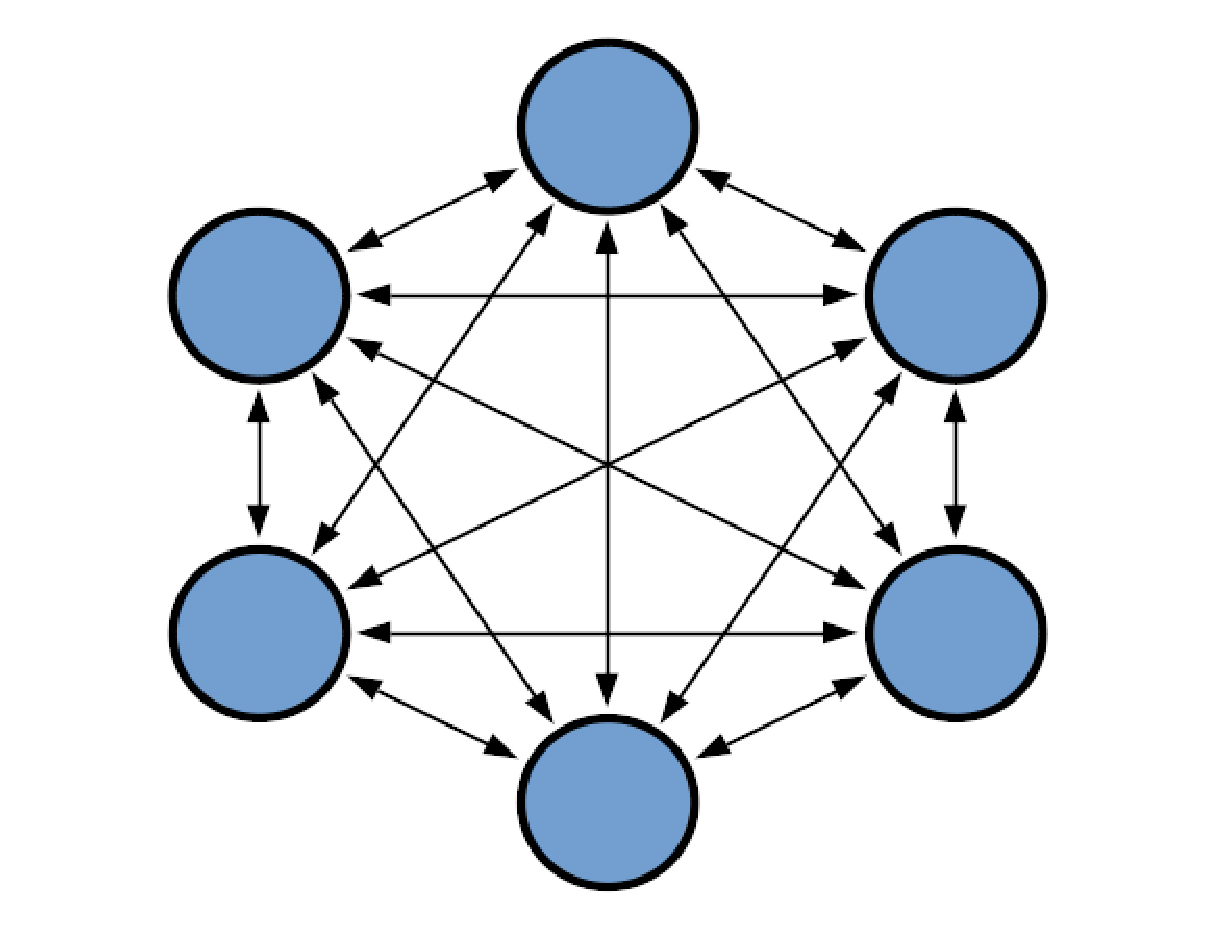
\includegraphics[width=50mm]{pht/DistributedSystem.eps}
    \caption{分散システム}
    \label{fig:DistributedSystem}
  \end{minipage}
\end{figure}

\begin{figure}[h]%挿入図
  \begin{center}
    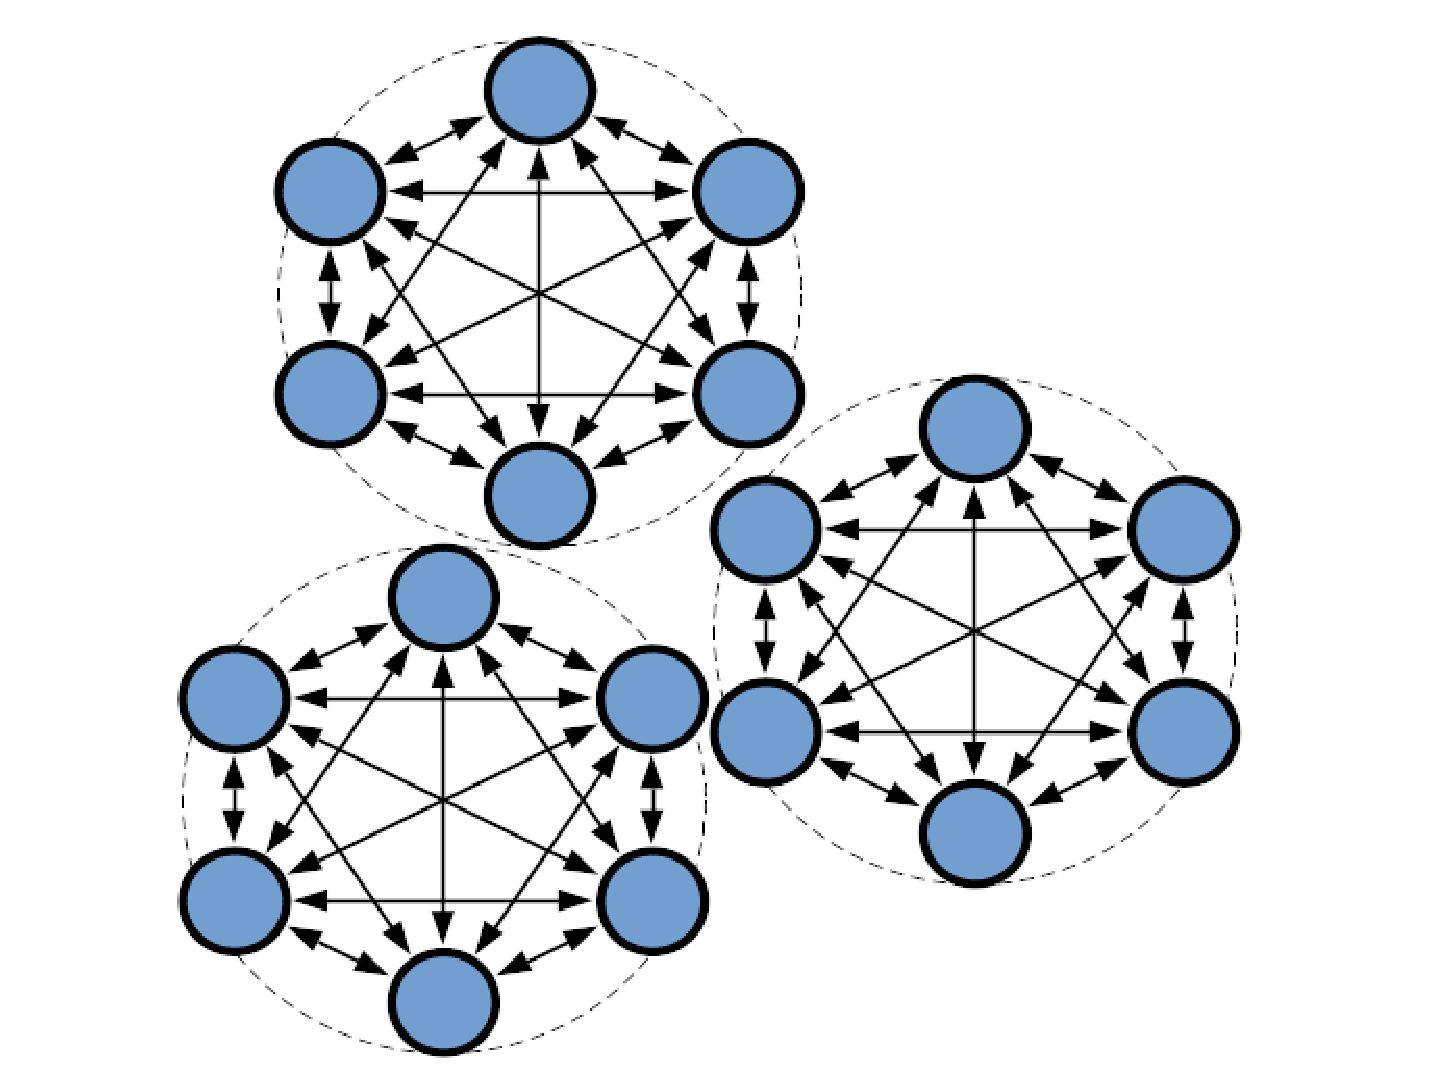
\includegraphics[width=100mm]{pht/DomainSplit.eps}
  \end{center}
  \caption{ドメイン分割}
  \label{fig:DomainSplit}
\end{figure}

図のように,集中システムは1つの中心があり,そこにほかのコンピューターが接続する形になっており,分
散システムは複数のコンピューター同士が相互に接続し合って形成される.
システムによっては,分散システムと集中システムを組み合わせることもあり,
状況に応じて適切な構造を取るように工夫されてる.
集中システムでは,中心のコンピューターが動かなくなるとシステム全体が停止
(システムダウン)してしまう「単一障害点」と呼ばれるマシンが存在したり維持管理コストが
かかってしまったりする欠点があるものの,システムの柔軟性や一貫性を維持するのが比較的,容易である長所がある.
また何よりもシステムにおけるデータ完全性を維持できるメリットがある.
分散システムは,システムにおける処理の多くのコンピューターで分担するためコストを削減することがで,
単一障害点がないことでシステムダウンする可能性がとても低くなる利点がある.
加えて,計算能力を高めていくことも可能になる.
ネットワークに接続している多くのコンピューターの計算能力を利用できるため全体の計算能力を徐々に大きくすることや,
今では多くの人々が高性能のPCやスマートフォンなどを持つようになってるため,それらが接続し合って大きな計算能力を実現するようになった.
また低コストかつダウンしないシステム
分散システムは,複数のコンピューター同士が接続し合って形成される.
システムによっては,分散システムと集中システムを組み合わせることもあり,
状況に応じて適切な構造を採るように工夫されている.

%集中システムと分散システムそれぞれの長所・短所は表ーーーの通りであり
% 短所長所の表

\subsection{Bitcoin}
ブロックチェーンは2008年に「Satoshi Nakamoto」という仮名の人物
ないし集団が発表がたBitcoinの基幹技術として生まれ,現在は主に仮想通貨としての活用を目指す技術として注目を浴びている.
Bitcoinはデジタルマネーエコシステムの基礎となるコンセプトと技術の集合体である.
Bitcoinネットワークの参加者間で,価値の保有と転送がBitcoinという名の通貨単位で行われる.
ユーザー間の通信は主にBitcoinプロトコルに基づいて,インターネットを通じて行われる.
Bitcoinのプロトコルスタックはオープンソースとして利用可能であり,
ノートパソコンからスマートフォンまで,様々なデバイス上で動作する.

ユーザーはネットワークを通じてBitcoinをやり取りすることで,従来の通貨で行うほぼ全てのこと,つまり
物品の売買から個人や組織への送金,融資まで行うことが可能になる.
Bitcoin自体も売買が可能であり,専門の両替機関で他の通貨とも両替することも可能です.
Bitcoinは高速かつ安全であり,国境を越えて取引が可能であることから,
ある意味でインターネットに使うための最適な通貨とも言えるかもしれない.
伝統的な通貨と異なりBitcoinは完全に仮想的なものです.物理的なコインは存在せず,またデジタルコイン
自体が存在するわけでもありません.コインは「送信者から受信者へある一定量の額面を移動させる」という
取引(トランザクション)の中で示されるものである.

Bitcoinのユーザーはトランザクションの所有権を証明する鍵を所有し,そのトランザクションの中に記載さ
れた額面を使用したり新しい所有者に送金することができる.
この鍵はそれぞれの利用者のPC上の電子財布(ウォレット)に保持される.
この鍵の保有がBitcoinを使用する唯一の条件であり,そのコントロールは各ユーザーにゆだねられている.

Bitcoinは分散されたpeer-to-peerのシステムであり,何らかの"中央"サーバや管理者が存在するものではない.
Bitcoinは取引の過程で行われる"マイニング"と呼ばれる数学的な解を見つけ出す競争により新たに生み出される.
どの(フルプロトコルスタックを動作させている)Bitcoinネットワーク参加者も,
自身のコンピューターリソースを用いて取引の記録処理と検証処理を行うことでマイナーとなることができる.
平均して10分に1回の頻度で誰かが数学的な解を見つけることで取引が検証され,
その解の発見者にはBitcoinが新たに与えられいる.
従ってBitcoinのマイニングとは,中央銀行が行う必要があった通貨の発行と決済の機能を,
世界的な競争で代替したものである.
Bitcoinプロトコルにはマイニングの機能を規定するアルゴリズムが組み込まれている.
マイナーが行わなければならないタスクの難易度は,マイナーの数(またはCPUの数)が変動しても
平均的に10分に1回ほど解が見つかるように自動的に調整されいる.
またプロトコルではBitcoinが新たに発行される頻度は4年毎に半減されるように規定されており,
またBitcoinの総発行量は2100万Bitcoinを超えないように規定されている.
その結果,Bitcoinの流通数は容易に予想可能で2140年に2100万に到達するカーブを描くことになる.
Bitcoinはプロトコル名でもありネットワーク名でもあり,
さらには,分散コンピューティングのイノベーションの名称でもある.

\subsection{ブロックチェーン}

ブロックチェーンは2008年に「Satoshi Nakamoto」という仮名の人物
ないし集団が発表がたBitcoinの基幹技術として生まれ,現在は主に仮想通貨としての活用を目指す技術として注目を浴びた.
デジタル通貨システム「Bitcoin(ビットコイン)」を実現するための分散タイムスタンプとして提案された.
ビットコインは,管理者のいない環境下で電子的に表現された通貨の制御権の移転,すなわち送金を妨害されないことを目標に設計されている.
送金の取引は入金(入力)と出金(出力)の間の関係を記述するが,
ビットコインでは,未使用の取引出力がコインであるとするいわゆる

UTXO(Unspent TX Output)構造(図 -1)を用いて電子コインのデジタルデータ形式を定義している.
この構造は,適切な秘密鍵を用いて取引にディジタル署名できる主体だけが送金できることを保証するが,
署名の検証に必要な情報(公開鍵)をデータ構造の中に埋め込み,
公開鍵のメッセージダイジェスト(ハッシュ値)をコインの送金の宛先とすることで,
まったく関係のない第三者でも公開鍵の正当性を確認でき,取引の形式的な正しさを検証可能にした点である.

仮想通貨のひとつであるビットコインは,ブロックチェーンによって通貨の取引を管理するが,
そこで利用されている暗号学的ハッシュ関数は,
$SHA-256$と$RIPEMD160$である.ブロックチェーンとは,通貨の取引履歴のように改ざんされないよう
管理されるべきデータを扱うための,分散型($P2P$型)の台帳を実現するための技術である.

%\subsubsection{ブロックチェーンの構造}

%ブロックチェーンは「ブロック」と呼ばれるデータを数珠状につないだ形を
%しており,ブロックを要約したブロックに取り込むことで全体の整合性を取っている.

%\subsubsection{ブロックチェーンの非中央集権性}
%ブロックチェーンの中央集権性

%\subsubsection{ブロックチェーンの改ざん耐性}

      \subsection*{ビットコインにおけるブロック構造}
一定数のトランザクションを格納したものをブロックを呼ぶ.
ブロックには,多数のトランザクションとあとで説明する「ナンス」(Nonce)と呼ばれる特別な値,そして直前のブロックのハッシュ値を持っている.
「ブロック」に含まれた取引のみを「正しい取引」と認めることにする.
そしてネットワーク全体で「唯一のブロックの鎖」を持つようにする.
これによって「一貫した取引データを全体で共有できる」というのがブロックチェーンの考えである.%(図10.5)

ビットコインブロックチェーンにおけるブロック構造は以下図のように構成されている.
%図を作成する.-------------------------


            \subsubsection{transaction(トランザクション)}
トランザクション
            \subsubsection{Nonce(ナンス)}

            \subsubsection{hash値(ハッシュ値)}


      \subsection{P2Pネットワーク [peer to peer NetWork]}%ブロックチェーンの教科書
P2Pネットワークは,Peer(ピア)と呼ばれる対等な立場のコンピューター同士が相互にデータを融通し合って形成されるネットワークです.
%図2.5
P2Pネットワークの性質として,
\begin{enumerate}
  \item 「システムがダウンしない」
  
  \item 「ネットワークの分断耐性が強い」
  
  \item 「データの一貫性を維持することが難しい」
  \end{enumerate}
という点が挙げられる.


      \subsection*{Proof of Work (PoW)}%ブロックチェーンの教科書
不特定多数のコンピューターによる演算を行いブロックチェーン全体の整合性を保つためのアルゴリズム
具体的には,取引データを要約したデータやタイムスタンプなどのデータをひとまとめにしそのデータにナンス(Nonce)を加えて,ハッシュ関数にかけてハッシュ値を求める.
このハッシュ値が一定値(目標値)よりも小さな値になるまでナンスを変えて計算する.
このことを「マイニング」と言い,マイニングを行う主体をマイナーと呼ぶ.

%PoWのおおまかなプロセス図

ナンス以外のデータは固定されているので,ナンスの値を少しずつ変えるだけになる.
しかし,ハッシュ関数の性質から入力値(ナンスの値)が変化するだけでも,出力させるハッシュ値は大きく変動する.
そのため,マイナー,一定の値よりも小さくするため,ナンスの値を推測することは基本的にできません.
従って,PoWを行い報酬をもらうマイナーは,ナンスの総当り計算をするしか方法がない
条件(難易度)に合うナンスを見つけるとマイニング成功となり,成功したマイナーはマイニング報酬を受け取ることできる.

ブロックに対してハッシュ値を計算する際に,先頭から特定の個数$0$が並ぶようなハッシュ値を,ナンスという値を変えながら探していくという作業である.
ハッシュ値の計算は,逆算ができない性質を持つことにより,特定の性質を持つハッシュ値となるよう1つ1つ計算して見つけるしかない.

従って,非常に大規模な計算が必要となる.この作業により見つけられた先頭から特定の個数$0$が並ぶハッシュ値を持ったブロックだけをネットワーク全体で「正しいブロック」として認める.
ハッシュ値の先頭から並ぶ$0$の数は,多ければ計算が難しく,少なければ容易となる.
ビットコインでは,およそ$10$分に$1$回の頻度で条件を満たすハッシュ値を見つけられる程度の個数に調整されている.
これは,コンピュータの性能向上やユーザ数の増加に応じて変更される.


PoWの大まかなプロセスは以下の通り
\begin{itemize}
  \item ネットワーク上を伝搬する取引データを受信して記録しておく.
  \item トランザクションをまとめてブロックを生成する.
  \item ナンスの値を少しずつ変えながら大量のハッシュ計算しナンス値を探索を行う.
  \item 条件に合うナンス値を見つけた人がブロックを完成させてほかのノードに報告する.
  \item ほかのノードはブロックの中身とナンス値が正しいかどうか検証する.
  \item ナンス値が正しければ,ブロックを完成させた人に報酬が支払われる.
\end{itemize}

difficultyターゲットを満たすSHA256のアルゴリズムに対し,解を見つけなければなりません.

      \subsection*{暗号学的ハッシュ関数} %(参考@分散システム31第2班)

暗号の利用方法の1つに,メッセージの完全性を確認するための情報であるメッセージダイジェストと呼ばれる固定長のビット列を生成するものがある.
任意の長さのメッセージから固定長のビット列を生成する暗号アルゴリズムは,暗号学的ハッシュ関数と呼ばれる.

暗号学的ハッシュ関数は,以下の性質を持つ.
\begin{itemize}
  \item 原像計算困難性
  \item 第2原像計算困難性
  \item 衝突困難性
\end{itemize}

原像計算困難性とは,ハッシュ値$h$が与えられたとき,$ h = hash(m)$となるような任意のメッセージ$m$を探すことが困難な性質である.

第2原像計算困難性とは,入力$m1$が与えられたとき,$ hash(m1) = hash(m2)$ となるようなもう1つの入力$m2$($m1$とは異なる入力)を
見つけることが困難である性質である.

衝突困難性とは,$hash(m1)= hash(m2)$となるような2つの異なるメッセージ$m1$と$m2$の組を探すことが困難である性質である.
これらの性質によって,2つのメッセージに対するダイジェストが同じである場合,メッセージが同一である可能性が高いことを意味する.

また,逆にダイジェストが異なる場合は,メッセージは異なるものであることを意味する.

文書の完全性を保証する情報としては,メッセージダイジェストが用いられる.
メッセージダイジェストは入力文書の大きさのよらない固定長の情報(ハッシュ値)であり,以下の特徴を持つ.

\begin{itemize}
  \item メッセージからメッセージダイジェストが簡単に計算できる.
  \item メッセージダイジェストからメッセージを見つけることは出来ない.
  \item メッセージから同じメッセージダイジェストが生成される別のメッセージを見つけることはできない.
  \item メッセージを1ビットでも変更すれば,メッセージダイジェストは全く異なる値になる.
\end{itemize}

このような特徴を持つメッセージダイジェストを生成するアルゴリズムとして,$MD5$,$SHA-1$などのハッシュアルゴリズムが
従来から使われてきたが,$MD5$はすでに破られており,$SHA-1$についても脆弱性が指摘されている.
現在は,$SHA-2(SHA-256)$あるいはその後継として公募された$SHA-3$への移行が急がれている.

\subsection*{ビットコインにおけるブロック構造}
ビットコインブロックチェーンにおけるブロック構造は以下図のように構成されている.

	Version	ソフトウェア/プロトコルのバージョン番号
	Previous Block Hash	親ブロック(1つ前のブロック)のハッシュ値
	Merkle Root	ブロック内の全トランザクションに対するマークルツリーのルートハッシュ
	Timestamp	ブロックの生成時刻
	Difficulty Target	ブロック生成時のProof of Workのdifficulty
	Nonce	Proof of Workで用いるカウンタ
\begin{itemize}
    \item transaction(トランザクション)
    \item Previous Block Hash
    \item Merkle Root
    \item Timestamp
    \item Difficulty Target
    \item Nonce
\end{itemize}

      \subsection*{ハッシュレート}
本研究での,ハッシュレートとは,単位時間あたりに暗号学的ハッシュ関数の計算を行うことができる回数である.
この時の改ざん耐性は,マイニングに勝利してブロックを生成するのは,ハッシュレートが
最も能力のあるノードである為,ハッシュレートの最大値のノードが基本的にマイニングに勝利し報酬を受け取ることができる.

      \subsection*{公開鍵暗号方式}

公開暗号方式では,暗号化と復号でそれぞれ異なる鍵を使う.秘密鍵と公開鍵が利用され,秘密鍵は自分だけが持っており他者に教えてはいけない鍵.
公開鍵は広く公開している鍵とそれぞれの役割が異なっている.
ここで,秘密鍵と公開鍵の重要な特徴として,公開鍵から秘密鍵が逆算されないことが挙げられ,
そうでなければ,人に教えてはいけない情報を,誰もが知っている公開鍵から特定されてしまい,暗号技術として成り立たなる.
ビットコインブロックチェーンでは公開鍵暗号方式が使われており,アドレスの生成や取引データのやり取りなど,様々な場面で利用されている.

      \subsection*{共通暗号方式}
共通暗号方式は,暗号化と複合で同じ鍵を用いるため,鍵を安全に相手と共有する必要がある.
また共有する相手の数だけ鍵が必要なため相手が増えれば増えるほど管理が煩雑になるデメリットがある.
このデメリットを回避するために,公開暗号方式が開発された.

      \subsection*{楕円曲線暗号}
楕円曲線暗号は1980年代半ばに提案された暗号方式で楕円曲線という特殊な曲線を利用している.
暗号アルゴリズムはコンピューターの処理性能の向上や攻撃手法の高度化によって日々脅威にさらされている.
そのため,利便性を保ちつつ,高い安全性を維持する方法が常に検討されている.


\subsection{スケーラビリティ問題へのアプローチ方法}
スケーラビリティの問題へのアプローチとしていくつか研究として行われている.


\subsubsection{オフチェーン ( off-chain )}
Lightning Network[6]のようなオフチェーンスケーリング技術が注目されることが多い.
しかし,オフチェーン取引はブロックチェーン上に記録を残さないため,監査可能性を最大化するというビットコインの本来の考えから遠ざかっている.

          \subsubsection{オンチェーン ( on-chain )}
オンチェーンのスケーラビリティ問題を解決するためには,
ブロックサイズを大きくするか,ブロック生成の時間間隔を短くする2つのアプローチで行われている.

/subsection{}

      \subsection{ブロックチェーンコアノードのドメイン分割}
ブロックチェーンコアノードの分割は,文献 \cite{fujihara1}\cite{fujihara2}で提案されている.
この提案手法に基づいて本研究は進める.
地理的に近いコアノード間で自律的にドメインを形成し,ドメインごとに固有のブロックチェーンを管理する方法が提案されている[7, 8, 9].この
しかし,各ドメインのコアノード数が減少すると,ブロックチェーンの分散性や改ざん耐性が低下するという問題がある.

      \subsection*{電子署名}
通常の電子署名は秘密鍵が漏洩することによる改ざん
が可能であり,改ざんされたことの検知も不可能である.

一方,ヒステリシス署名では,電子署名が入れ子構造になって署名がされている為,
署名の改ざんを行う為には,改ざんした内容
以降の全ての入れ子構造になった署名を改ざんする必要があり,改ざんが著しく困難になる.
また,部分的に改ざんされた場合は,入れ子構造を検証することで,改ざんの検知も可能になる.
これはPoWに代わる改ざん耐性技術としてブロックチェーンが注目を集める前から知られており,
過去のデータ等を改ざん耐性を持たせて保存することができる.

      \subsection{ヒステリシス署名}

ヒステリシス署名は,過去の署名履歴を取り込みながら署名生成を行う方式である.

ヒステリシス署名\cite{suzaki}とは,通常の電子署名に連鎖する入れ子構造を持たせることで,
その改ざん耐性を向上させる技術である.
図\ref{fig:hysteresis}にヒステリシス署名の構造を示す.
1つ前のヒステリシス署名$S_{n-1}$を暗号学的ハッシュ関数にかけたハッシュ値$H(S_{n-1})$
と一緒に保存したい$m$個のデータ($B_{D_1}, \cdots, B_{D_m}$)のハッシュ値
($H(B_{D_1}), \cdots, H(B_{D_m})$)を追加する.この全体の署名$S_n$を更に追加して生成された
ものがヒステリシス署名となる.

\begin{figure}[H]%挿入図
  \begin{center}
    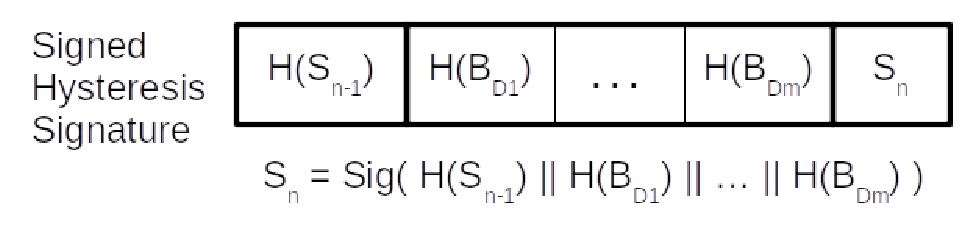
\includegraphics[width=100mm]{pht/hysteresis_signature.eps}
    %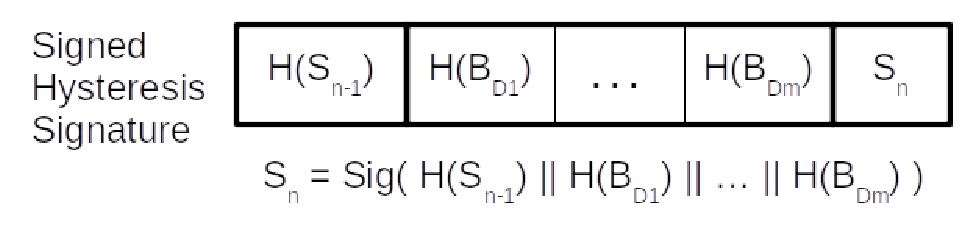
\includegraphics{pht/hysteresis_signature.eps}
  \end{center}
  \caption{ヒステリシス署名の例}
  \label{fig:hysteresis}
\end{figure}


これにより,有効期限のが切れた電子証明書に対応する電子署名であっても,有効期限内の電子署名書により
真正性が保証された電子署名空から連鎖構造を辿ることで,結果として真正性を証明可能となる.

なお通常の署名方式では,署名方式では,署名対象となるメッセージと電子署名とを組みにして相手の(検証者)に送るが,
ヒステリシス署名では,それに加えてひとつ前の署名結果のハッシュ値も合わせて送ることが可能になる.

時間情報を文書に織り込むのではなく,署名者が過去に関わった署名付き電子文書の圧縮データを次々に織り込んで行くことである.


%ヒステリシス署名は,直前に生成された電子署名のハッシュ値を取り込み,電子署名間に連鎖構造を持たせる
%署名である.これにより有効期限のが切れた電子証明書に対応する電子署名であっても,有効期限内の電子署名書により
%真正性が保証された電子署名空から連鎖構造を辿ることで,結果として真正性を証明可能となる.

%ヒステリシス署名とは,過去の署名履歴を取り込みながら署名生成を行う方式である.
%これにより署名間に連鎖構造を築き,暗号ブレイク時にも偽造を困難にする.
%ヒステリシス署名では,n回目の電子署名生成時にn-1回目の署名結果のデータのハッシュ値を作用させる.
%従ってある時でのデータは,当該署名しシステムを使用開始してからのすべての署名履歴が影響した値となっている

%なお通常の署名方式では,署名方式では,署名対象となるメッセージと電子署名とを組みにして相手の(検証者)に送るが,
%ヒステリシス署名では,それに加えてひとつ前の署名結果のハッシュ値も合わせて送ることが可能になる.


%電子署名技術が署名鍵の作成と解読における
%計算量の非対称性に依存する限り,コンピュータ技術の進歩により,
%暗号のブレイク状況,すなわち署名生成鍵を持っているエンティティが
%本来の鍵所持者以外にも存在するという可能性を確率的に有意とみなさざることを得なくなる
%状況が生じるこことは避けられない.
%これが電子署名アリバイ問題における基本的な状況設定である
%こうした状況でアリバイを実現するときの基本的な方法は,署名対象文書にその時間情報を織り込んで
%署名することである.

%しかし,そうした時間情報を再現可能なデータを織り込む限りでは,過去のに利用可能であった
%時間情報データを使って「過去の電子署名」偽造することは一般に可能となってしまう

%そしてこうした「過去の電子署名」偽造の可能性が存在する限り,調停者は電子署名のアリバイを承認することも崩すことも出来ない.

      \subsection{履歴交差法}
ヒステリシス署名の証明力はこうした
ヒステリシス署名つき文書が作成したエンティティの電子文書が署名を作成したエンティティの手を離れ,
他のエンティティの電子文書におけるヒステリシスとして署名に織り込まれた時に,さらに飛躍的に向上すると考えられる.
%参考テキスト図3

\subsection{Raft Consensus Algorithm}\cite{Raft Consensus Algorithm}
\label{Raft}
複数のノード間で合意を得る必要がある.
分散システムで合意するを得る手段にRaftがある
RaftはPaxosど同等の性能を持ちながらPaxosよりも格段の理解のしやすさを提供する分散合意プロトコルである.
%Paxosをあとで説明追加
Raftのアーキテクチャ概要を図1に示す.Raftを実行するノードには, LEADER,CANDIDATE,FOLLOWERという$3$種類の状態がる.LEADERはクラスタ内に1台しか存在しない.
クライアントは,LEADERノードとインタラクションする.クライアントはLEADERにアクセスしてきた場合はLEADERにリダイレクトされる.
FOLLOWERのノードはLEADERノードに従う.LEADERノードはクライアントノードから更新要求を受信すると,ログレコードを作成する.そしてLEADERノードはログレコードをストレージに保存した後,ログレコードをログレコードをFOLLOWERノードへ転送する.
FOLLOWERノードは受信したログレコードをストレージに保存すると,ACKをLEADERへ送信するLEADERを含め,Raftクラスタの過半数が命令を受け取ったことをLEADERが確認した後,クライアントにCOMMITを通知する.
最終的には,すべてのノードが同じ命令を同じ順番で実行するため,すべてのノードでデータが複製される.
即ちRaftは複製化状態機械に基づいて設計されている.一般に利活用されている複製化状態機械に例として,Chubby,ZooKeeperなどが挙げられる.
LEADERノードが故障したり,LEADERノードの故障したり,LEADERノードのネットワークコネクションが切断されると,Raftクラスタ内にLEADERが存在しなくなる.
このような場合,FOLLOWERノードは状態をCANDIDATEへと変更する.
クラスタ内のノードは各CANDIDATEへの投票を行い,新たなLEADERを選出する.
この選出にはクラスタを構成するノードの数の過半数の選任が必要である.
過半数を得たノードが存在しなければ,LAEDER選出作業を再実行する.

\newpage
%%----------------------------------------------------------------------
\section{ブロックチェーン履歴交差法}
%%----------------------------------------------------------------------
提案するブロックチェーン履歴交差法について説明する.
  \subsection{提案手法}
\label{teian}

本研究において提案するP2Pネットワークの構成を図 \ref{fig:p2p}に示す.
%
%
\begin{figure*}[H]%挿入図
  \begin{center}
    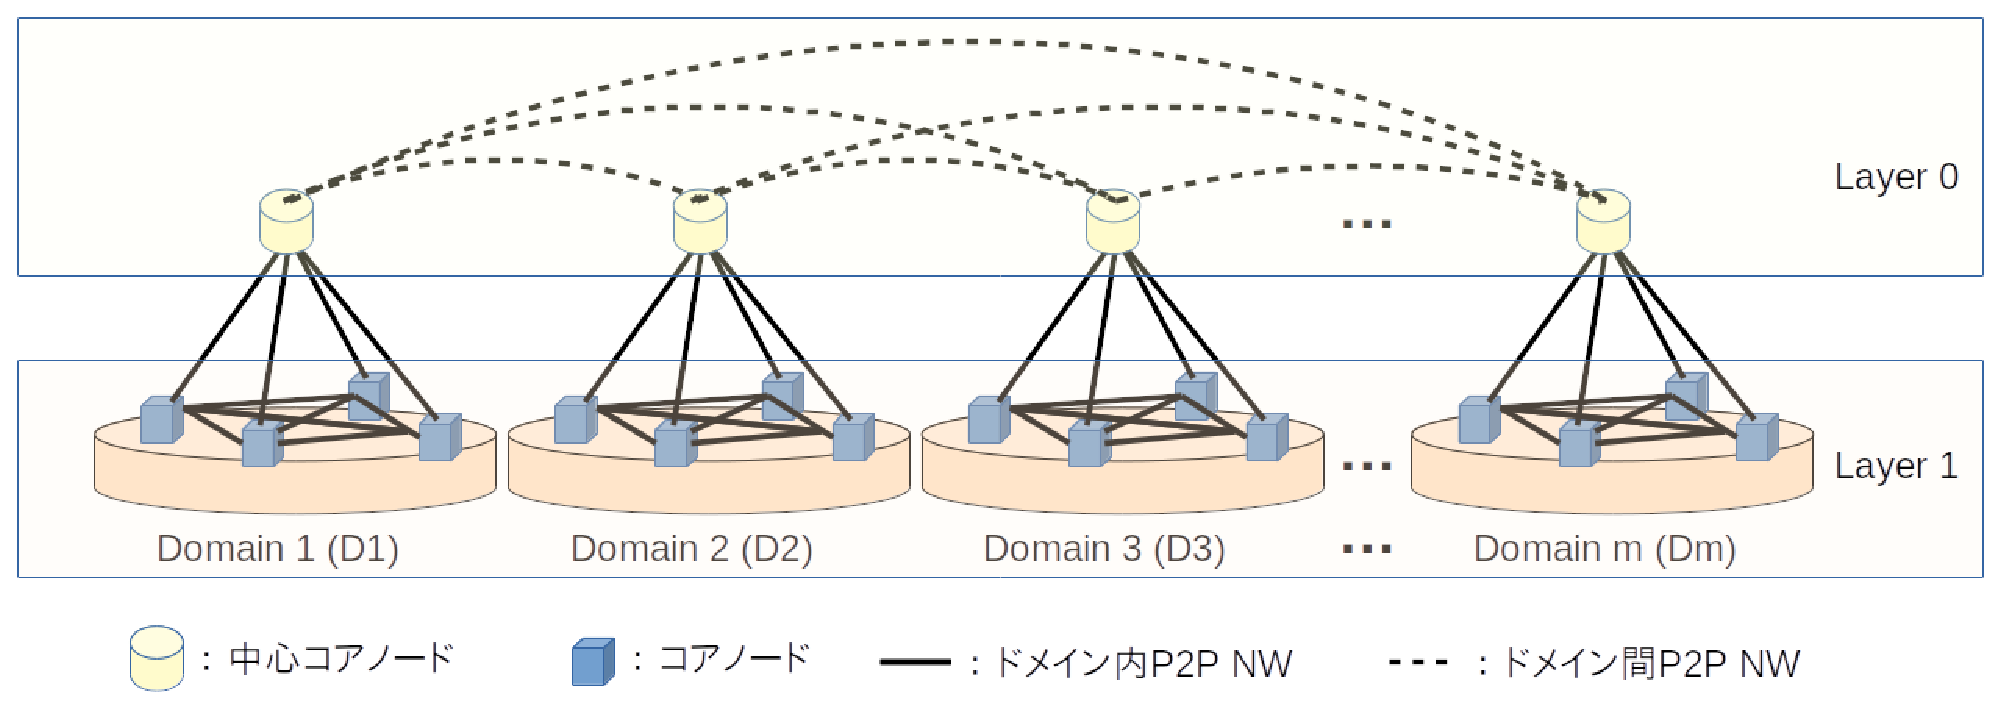
\includegraphics[width=130mm]{pht/p2p_network_image_r1.eps}
    %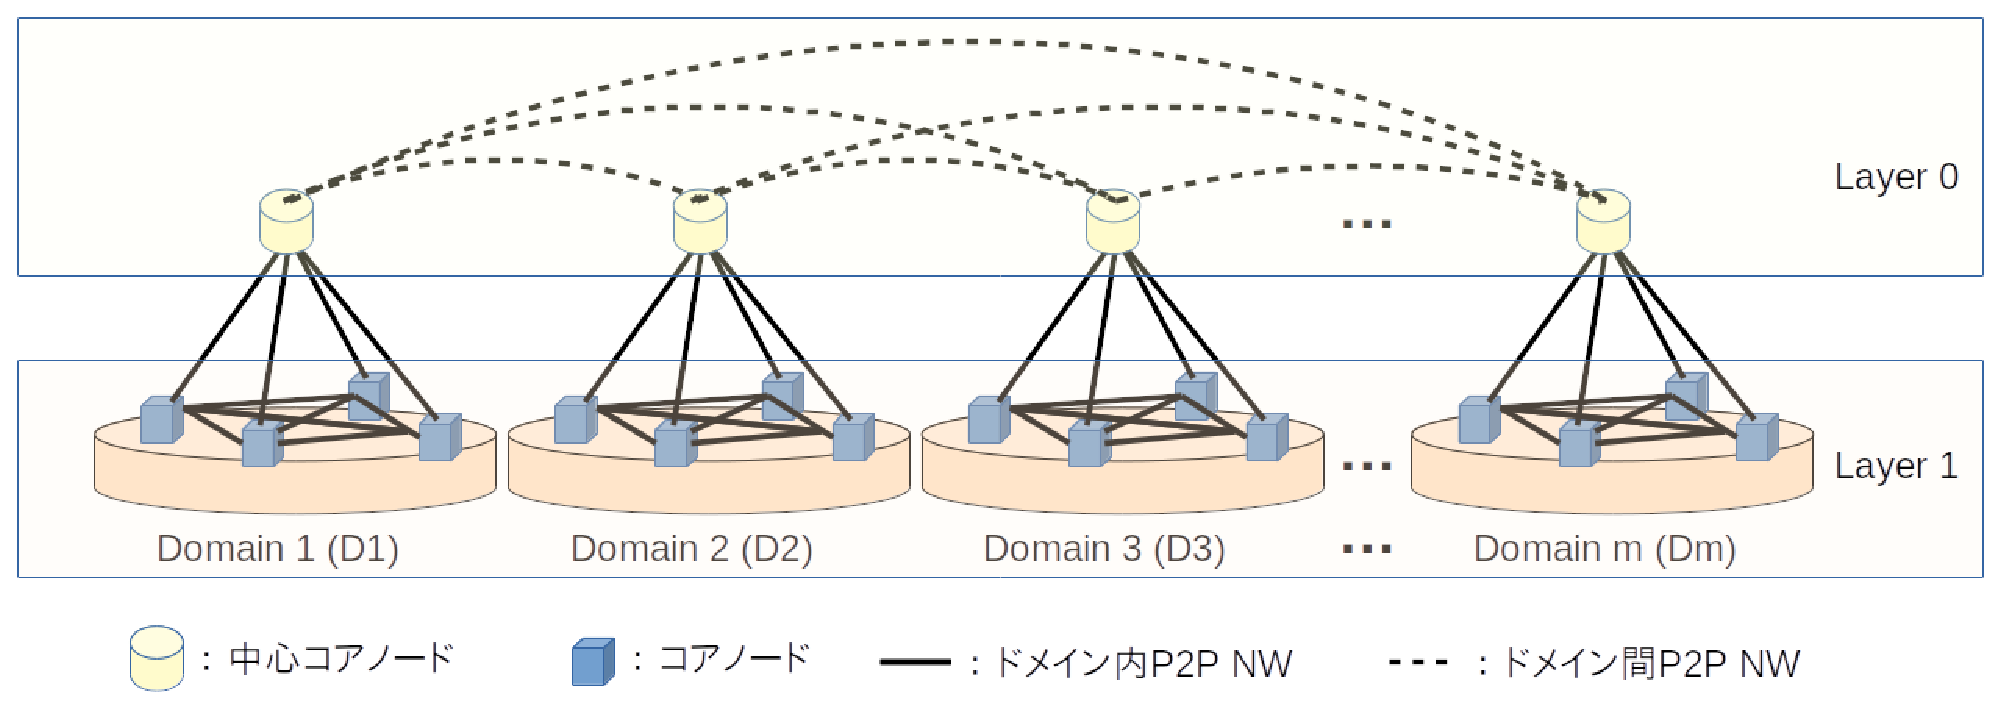
\includegraphics{pht/p2p_network_image_r1.eps}
  \end{center}
  \caption{P2Pネットワーク}
  \label{fig:p2p}
\end{figure*}


本研究におけるP2Pネットワーク環境は,Layer0と1のネットワーク層から構成される.
Layer1の層は通常のブロックチェーンを共有するP2Pネットワークである.
従来のブロックチェーンを共有しているP2Pネットワークに所属するノードの集合のことをドメインとして位置づけている.
本研究では,複数のドメインが互いにブロックチェーンに「指紋」としての役割を持つヒステリシス署名として共有する履歴交差法行うことで,
全ドメインの改ざん耐性での改ざん耐性向上を目指す.

Layer1では,各ドメイン ($D_1, D_2, \cdots, D_m$) が独自のブロックチェーンを管理する.
Layer0は,Layer1のドメインを代表する中心コアノード同士がLayer1とは異なる,Layer0のP2Pネットワークにより相互接続している.
%ここでは簡単の為,各ドメインの中心コアノードは1つとしているが,一般に複数あっても構わない.

\subsubsection{本研究におけるブロック構造}
提案するブロックの構造を図\ref{fig:block}に示す.
%
\begin{figure}[H]%挿入図
  \begin{center}
    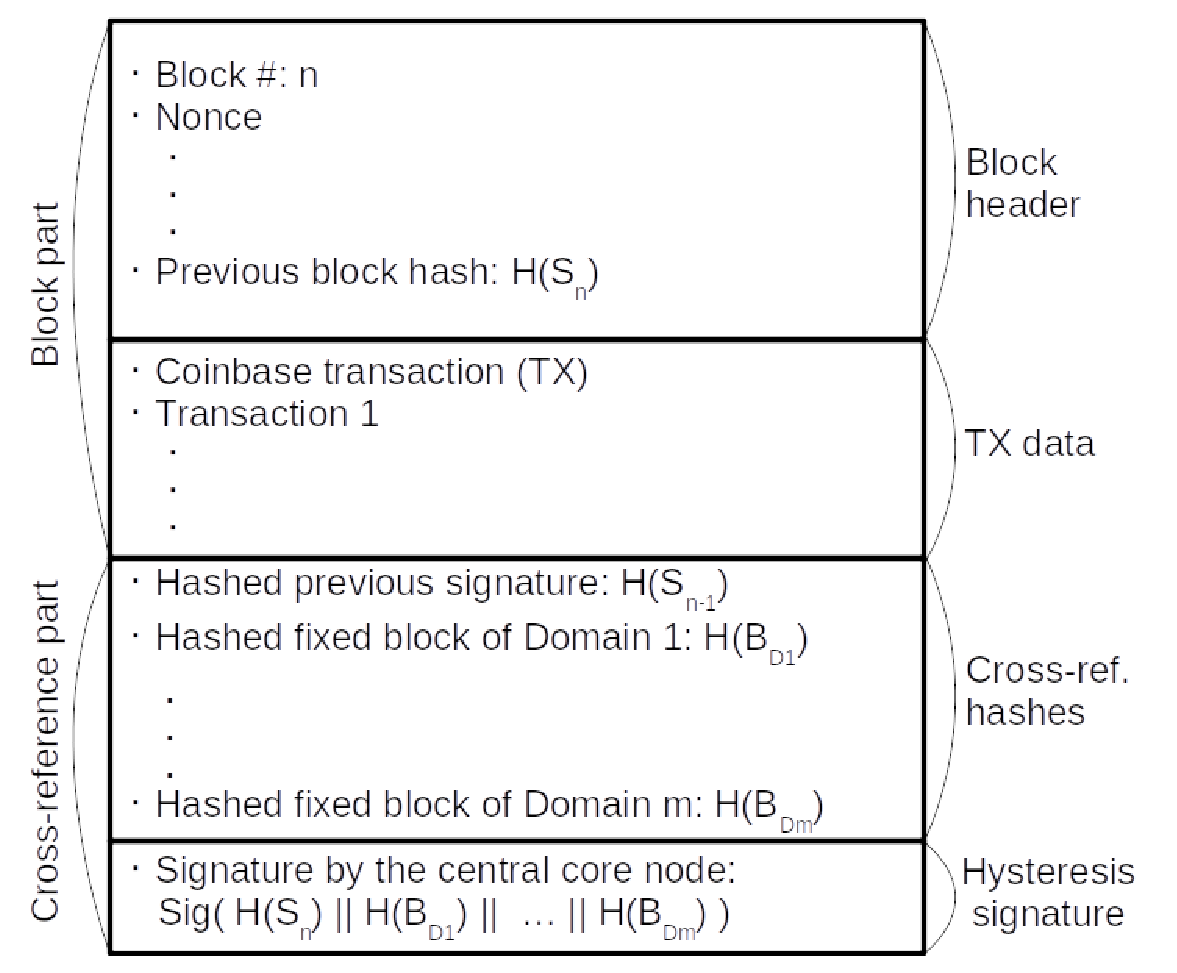
\includegraphics[width=100mm]{pht/block_structure.eps}
  \end{center}
  \caption{提案するブロック構造}
  \label{fig:block}
\end{figure}
%
従来のブロック構造に履歴交差部 (Cross-reference part) を追加する.
履歴交差部に書き込むヒステリシス署名は,Layer0を介して共有する.

\subsubsection{履歴交差法}
履歴交差法の動作アルゴリズム1を図\ref{fig:cross-ref}に示す.
%
\begin{figure}[H]%挿入図
  \begin{center}
    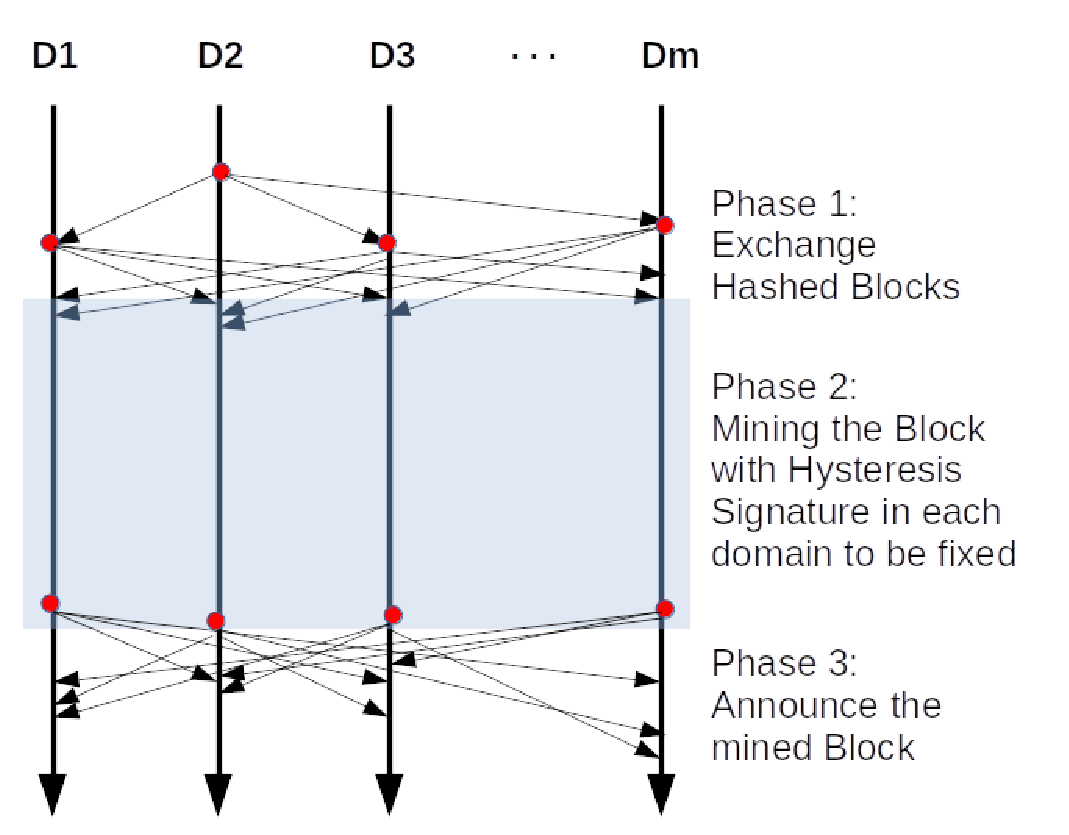
\includegraphics[width=120mm]{pht/time_sequence-algorithm1.eps}
  \end{center}
  \caption{提案する履歴交差法}
  \label{fig:cross-ref}
\end{figure}
%
全体の動作は,次の3つのPhaseから構成される.
以下にその流れを簡単に説明する.

\hspace{5mm}
%
\begin{enumerate}
    \item Phase1では,ドメイン間で$l$-確定ブロック(最新のブロックから 
          $l$ 個前のブロック)を含むメッセージをドメインを代表する
          中心コアノード同士で互いに送り合う(ただし$l$は正の整数).

    \item Phase2では,各ドメインが届いたメッセージを用いて図\ref{fig:hysteresis}
          のヒステリシス署名を行い,各ドメインが独立に署名を履歴交差部に書き込む
          為のマイニングを行う.(従来のマイニングと同様)

    \item Phase3では,マイニングし終えたブロックが,$l$-確定ブロックになったこと
          を他のドメインにブロードキャストして報告する.
\end{enumerate}
%
\hspace{5mm}
以上を提案する履歴交差法の一連の流れとし,履歴交差法を各ドメイン間で自律的に行う.

履歴交差法を実現する分散アルゴリズム\cite{manabe}を設計した.
その詳細を図 \ref{fig:algorithm1},\ref{fig:algorithm2}に示す.
本研究における履歴交差を実現する2つのアルゴリズムが正しく動作する前提条件として,次の1〜3が挙げられる.

\hspace{3mm}
%
\begin{enumerate}
    \item 中心コアノード同士が作るP2PNWは同期システムである.また,その構造は完全グラフとする.
    
    \item 中心コアノードは正しくアルゴリズムを実行し,互いに必ずブロックを転送する.
    
    \item アルゴリズム1では,全ての中心コアノードに故障停止がない場合に動作する.
    
    \item アルゴリズム2では,$t$-故障停止がある場合を想定する.
        つまり,最悪$t$個の中心コアノードが故障停止に陥った場合でも動作する.
\end{enumerate}
%
\hspace{3mm}
%
\begin{figure}[H]%挿入図
  \begin{center}
    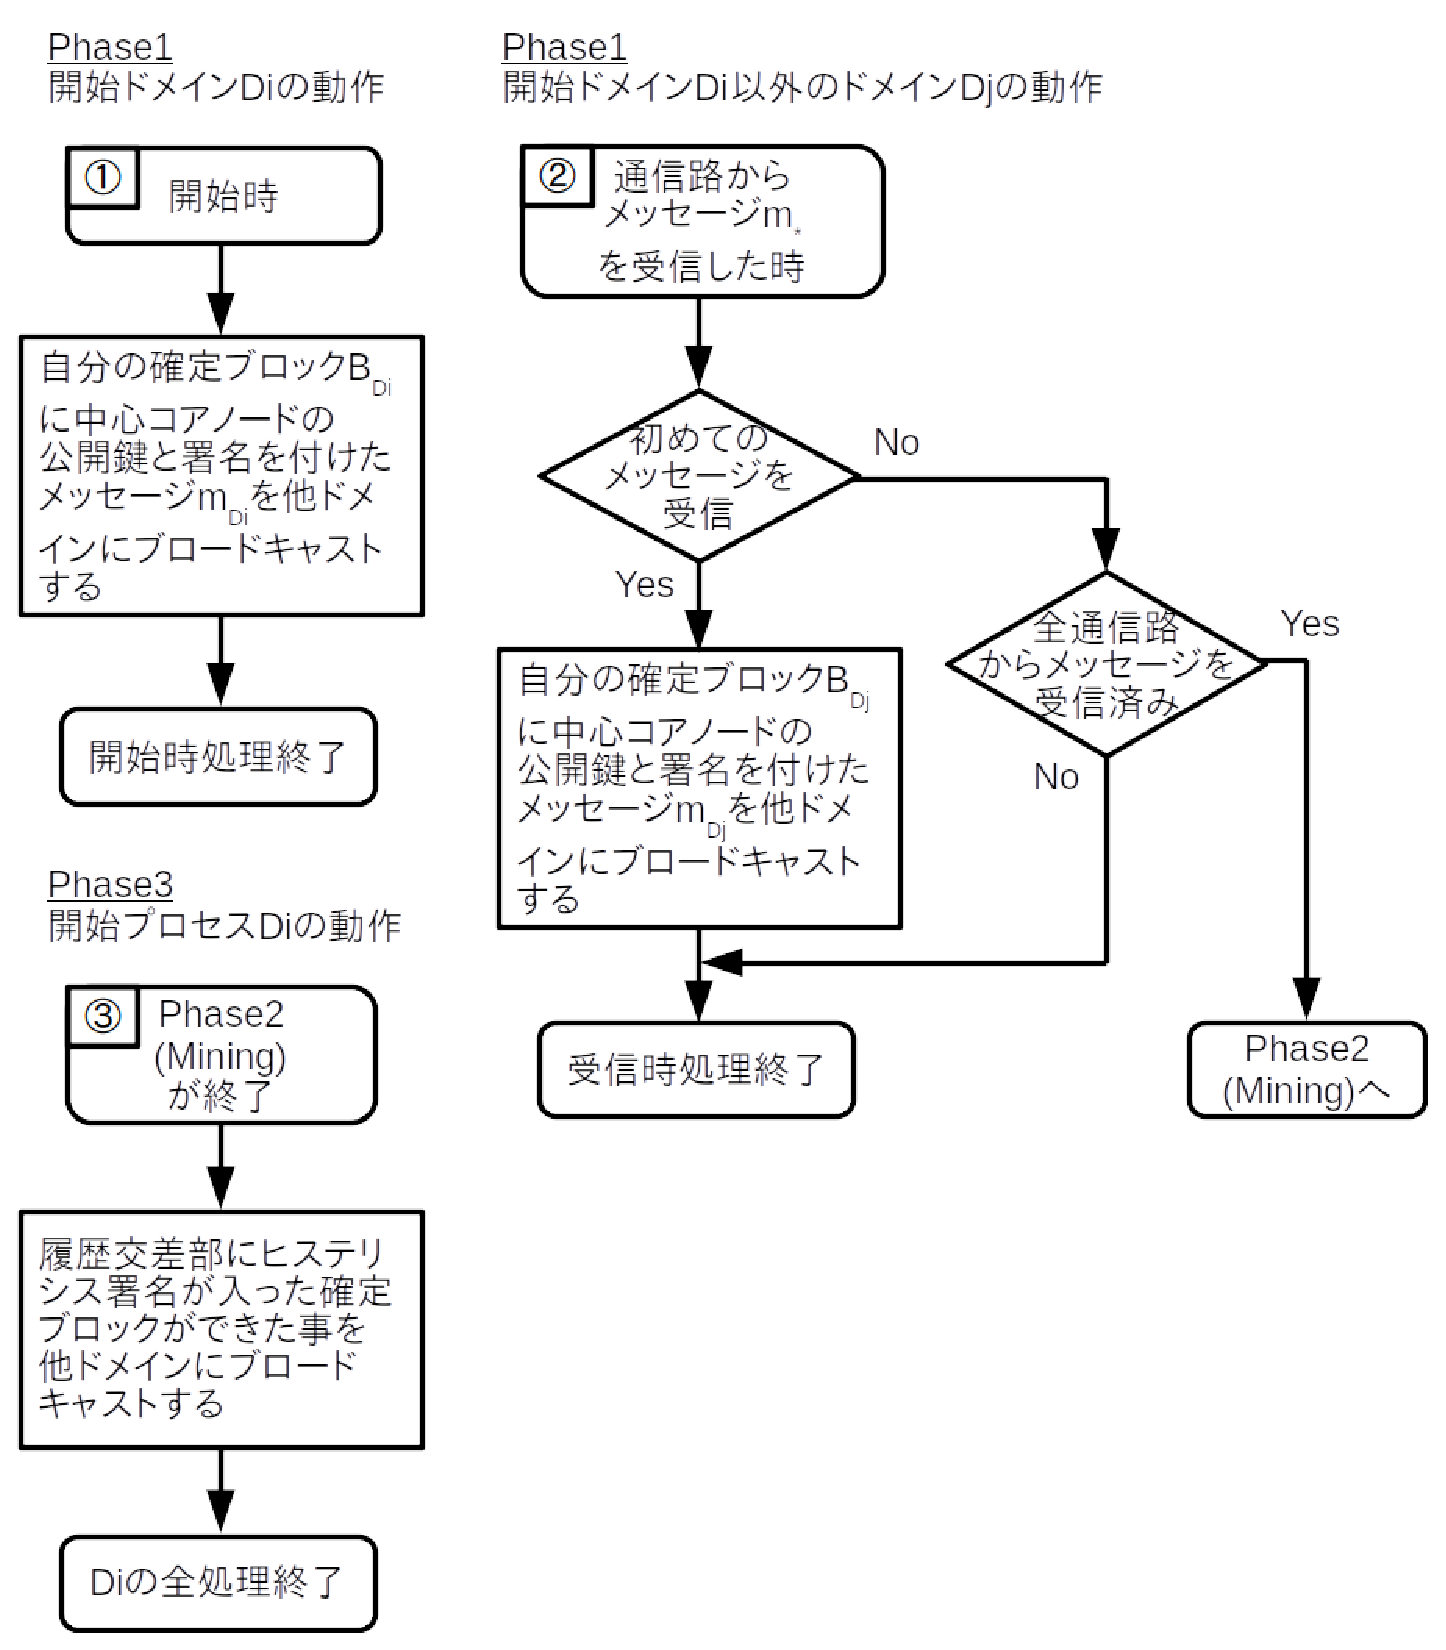
\includegraphics[width=100mm]{pht/flow_chart-algorithm1.eps}
  \end{center}
  \caption{アルゴリズム1(Phase 2はLayer1における通常のマイニング作業を行うだけである為,省略した.)}
  \label{fig:algorithm1}
\end{figure}
%
%
\begin{figure}[H]%挿入図
  \begin{center}
    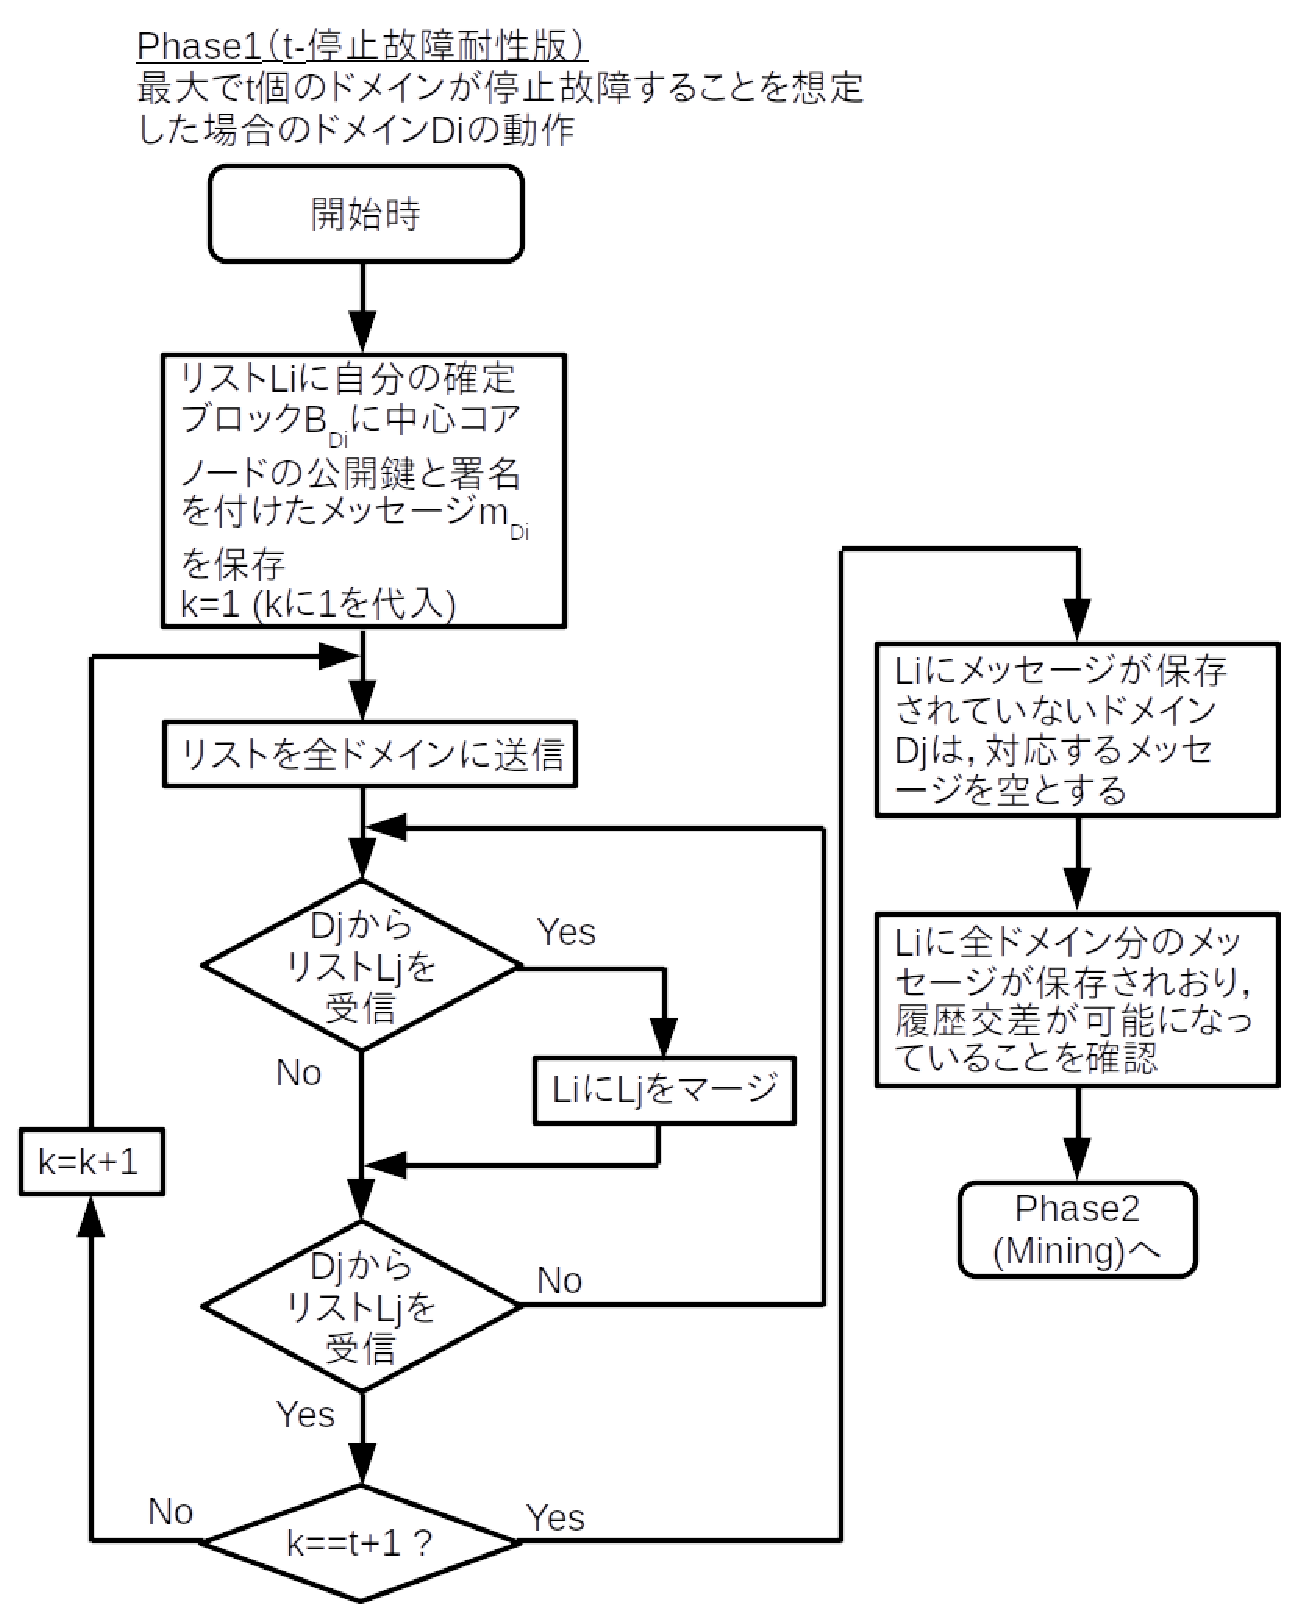
\includegraphics[width=100mm]{pht/flow_chart-algorithm2.eps}
  \end{center}
  \caption{アルゴリズム2(Phase 1のみを記述.その他のPhaseはアルゴリズム1と共通.)}
  \label{fig:algorithm2}
\end{figure}
%
      \subsubsection{提案方式の分散アルゴリズムの効率}%テキスト:分散処理システム
%関連研究で上に上げる必要がある.
通信計算量のとは,ある問題を解くアルゴリズムが開始してから終了するまでに送信されるメッセージの総数の最大値である.
最大値を評価する以外に,平均値での評価やメッセージの総数ではなくメッセージの総ビット数で評価することもある.
最大値で評価するのは最悪のケースを想定することを意味する.
 非同期な分散システムでは,計算が開始してから終了するまでの時間を評価することができない.
そこで,通信の遅れがプロセス内での計算よりも短いという仮定のもとで,次のような仮想的な同期実行を考える.
『第1ラウンドにおいて,各プロセスは同時に実行を開始し,内部計算およびほかのプロセスへの送信を実行し,ほかのプロセスからのメッセージ受信待ちになるまで動作を行う.
第$n + 1$ラウンドでは,第$n$ラウンドで送信されたメッセージがすべて受信側プロセスに到着する.各プロセスはそれらのメッセージを受信し,
受信したあとに実行する内部計算およびほかのプロセスからのメッセージ受信待ちになるまで動作を行う.』
このように動作を行った場合のラウンド数を時間計算量という.
時間計算量という.同様に時間計算量においても,最悪値や平均値で評価する.

分散アルゴリズムの効率は,通信計算量と時間計算量で評価することが一般的である.
提案した手法の分散アルゴリズム1,2の効率は,
アルゴリズム1が開始してから終了するまでに送信される通信計算量は$O(m^2 \cdot b)$,
アルゴリズム2の通信計算量は$O((t+1)(m^2 \cdot b))$となる.
また動作を行った場合の時間計算量は,アルゴリズム1は,$ T_1 + T_2 + T_3 $,
アルゴリズム2は$ ( t + 1 ) T_1 + T_2 + T_3 $ となる.
ここで $T_i (i=1, 2, 3)$は,アルゴリズム 1においてPhase $i$にかかる時間である.

\subsection{履歴交差法の理論的性能}

履歴交差法を行うことで,ブロックチェーンの改ざん耐性が向上することが期待される.
全世界のコアノードで管理するビットコインブロックチェーン方式と
近接するコアノードでドメインを形成位し,履歴交差法を用いた方式で
改ざん耐性向上比率を定義し,理論的にその比率を評価する.
全世界ノード数$N$で,ノード$i$のハッシュレートを$h_i$とする.
%ここで,ハッシュレートとは,単位時間あたりに暗号学的ハッシュ関数の計算を行うことができる回数である.
%前節で説明していれば,省略してもいいと思う.
この時の改ざん耐性は,マイニングに勝利してブロックを生成することができるのは,ハッシュレートが最も
大きなノードである為,ハッシュレートの最大値与えられる.
%
\begin{equation}
  \max(h_1, h_2, \cdots, h_N)
\end{equation}
%
ドメイン数が$m$個で,各ドメインに所属するノードの数が$D_m$個の場合を考える.
各ドメインの改ざん耐性は,ドメインに属するノードのハッシュパワーの最大値で与えられる.
%
\begin{eqnarray}
	A_1 &=& \max (h_{11}, \cdots ,h_{1D1}), \\
	A_2 &=& \max(h_{21}, \cdots ,h_{2D2}), \\
	    & & \vdots \nonumber \\
	A_m &=& \max(h_{m1}, \cdots ,h_{mDm})
\end{eqnarray}
%

%ここよくわからない.あとで検討
このドメインの中でハッシュレートが最大のノードがドメインが履歴交差法に参加する
インセンティブとなるように,全ドメインの中でハッシュパワーが最大のものと比較する.
%
\begin{equation}
A = \max(A_1, A_2, \cdots, A_m)
\end{equation}
%
上記の$m$個のドメインで履歴交差法を実行すると,全てのドメインのブロックチェーンを改ざんしない限り,
履歴交差部にヒステリシス署名の証拠が残ってしまう為,改ざんが検出されてしまう.
従って,改ざん耐性は全ドメインの最大ハッシュレートの和で表される.
%
\begin{equation}
	B = \sum_{i=1}^{m} A_i
\end{equation}
%
以上より,ドメイン$i$が履歴交差法に参加することで,期待される改ざん耐性向上比率$R_i$は次式で表される.
%
\begin{equation}
	R_i = \frac{B}{A_i} > 1 \hspace{5mm} (i=1, \cdots, m)
\end{equation}
%
また,ハッシュレートが最大のドメインが履歴交差法に参加することで期待される改ざん耐性向上比率$R$は次式で表される.
%
\begin{equation}
	(R_i \ge) R = \frac{B}{A} > 1  \hspace{5mm} (i=1, \cdots, m)
\end{equation}
%
このように,理論的には全てのドメインで改ざん耐性向上率を見積もることができる.

ここで,改ざん耐性向上率$R$を見積もる為に,ハッシュレートをランダムに割り振って乱数シミュレーションを行うことにより,数値的に評価する.
全ノード数を1万とし,ドメイン毎に分割されたノード数を一律 10, 100, 1000ノードとした場合を評価した.
全ノード数を1000万ノードとし,ドメイン毎に分割されたノード数を一律 10, 100, 1000ノードとした場合のハッシュレート$ h_{ij} $ ($i$:ドメイン番号,$j$:ドメイン内のノード番号)を次式であわらされるパレート分布とした.
%
\begin{equation}
	P(h_{ij}) = \frac{\alpha}{h_{ij}^{1+\alpha}} (h_{ij} > 1).
\end{equation}
%
ここで,$\alpha$はパレート分布のスケールパラメータである.
この値が小さいほどハッシュレートに格差が大きくなる.一般にハッシュレートはCPUの数に比例する.
CPUをいくつ購入できるかは,ノードを所持する人物ないしはグループの資本と関係している為,富の分布と相関があると予想できる.
この理由により,ハッシュレートの分布をパレート分布とすることは妥当であると考える.
シミュレーションの実行結果を図 \ref{fig:alpha2}, \ref{fig:alpha3}に示す.

一般にドメイン数が増加するほど,改ざん耐性向上比率$R$の分布のピークが
大きい方にシフトすることが分かる.また,ドメイン数が増えると分布の分散
も大きくなることが確認できる.
また図\ref{fig:alpha2}と図\ref{fig:alpha3}の比較により,スケールパラメータ
$\alpha$が小さくなるほど,改ざん耐性向上比率$R$の分布のピークが小さい方にシフトすることも分かる.

%
\begin{figure}[th]%挿入図
  \begin{center}
    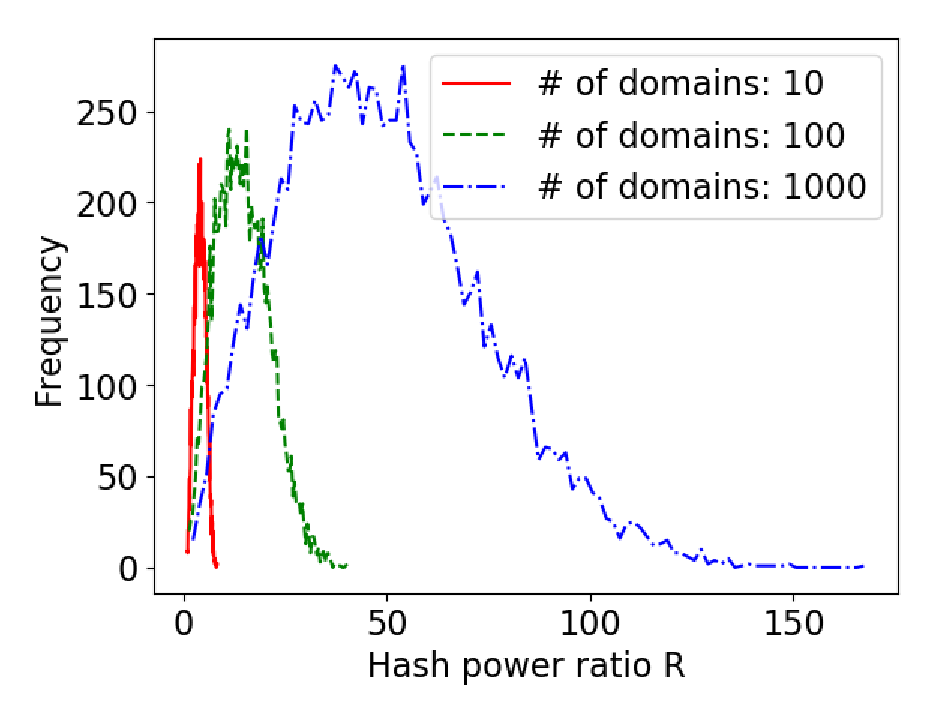
\includegraphics[width=100mm]{pht/hist-comp-R-alpha2.0-m1.0.eps}
  \end{center}
  \caption{改ざん耐性向上比率$R$の確率分布 ( $\alpha=2$の場合 ) }
  \label{fig:alpha2}
\end{figure}
%
%
\begin{figure}[H]%挿入図
  \begin{center}
    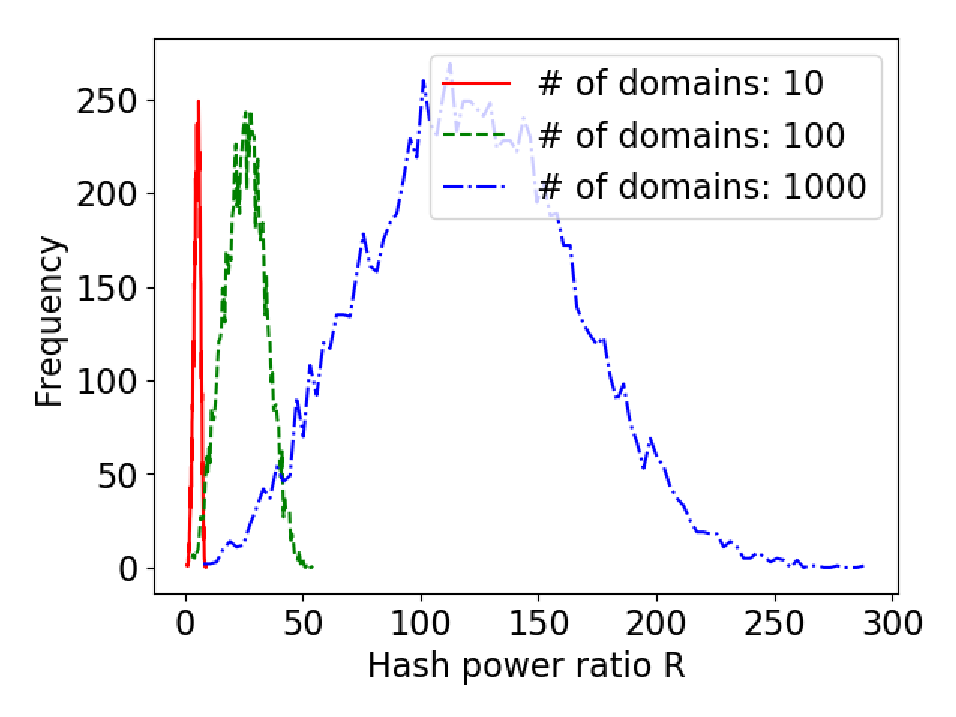
\includegraphics[width=100mm]{pht/hist-comp-R-alpha3.0-m1.0.eps}
  \end{center}
  \caption{改ざん耐性向上比率$R$の確率分布 ( $\alpha=3$の場合 ) }
  \label{fig:alpha3}
\end{figure}
%
\newpage
%

%--------------------------------------------------------------------------------理論的性能評価
%--------------------------------------------------------------------------------以下実装
\section{実装と実験}
\subsection{実装}
提案する手法を実現するコアノード実装に当たりLayer0における通信プロトコルの設計を行った.
\subsubsection{通信プロトコルの実装}
\label{syuhou}
Layer0における中心コアノード同士が履歴交差法を行うための
実装した通信プロトコルを以下に示す.

\hspace{5mm}
%
\begin{enumerate}
\item \textbf{MSG\_REQUEST\_CROSS\_REFERENCE}\\
\hspace{12mm} (履歴交差の依頼 )
\item \textbf{MSG\_ACCEPT\_CROSS\_REFFERENCE}\\
\hspace{12mm}  (履歴交差依頼の承認 )
  \item \textbf{MSG\_START\_CROSS\_REFFERENCE}\\
\hspace{12mm}  (履歴交差の開始号令 )
  \item \textbf{MSG\_CROSS\_REFFERENCE}\\
\hspace{12mm}  (履歴交差を行いたいblock内容の共有 )
  \item \textbf{MSG\_COMPLETE\_CROSS\_REFERENCE}\\
\hspace{12mm}  (履歴交差の完了通知 )
\end{enumerate}
%
\hspace{5mm}
%
\begin{figure*}[H]%挿入図
  \begin{center}
    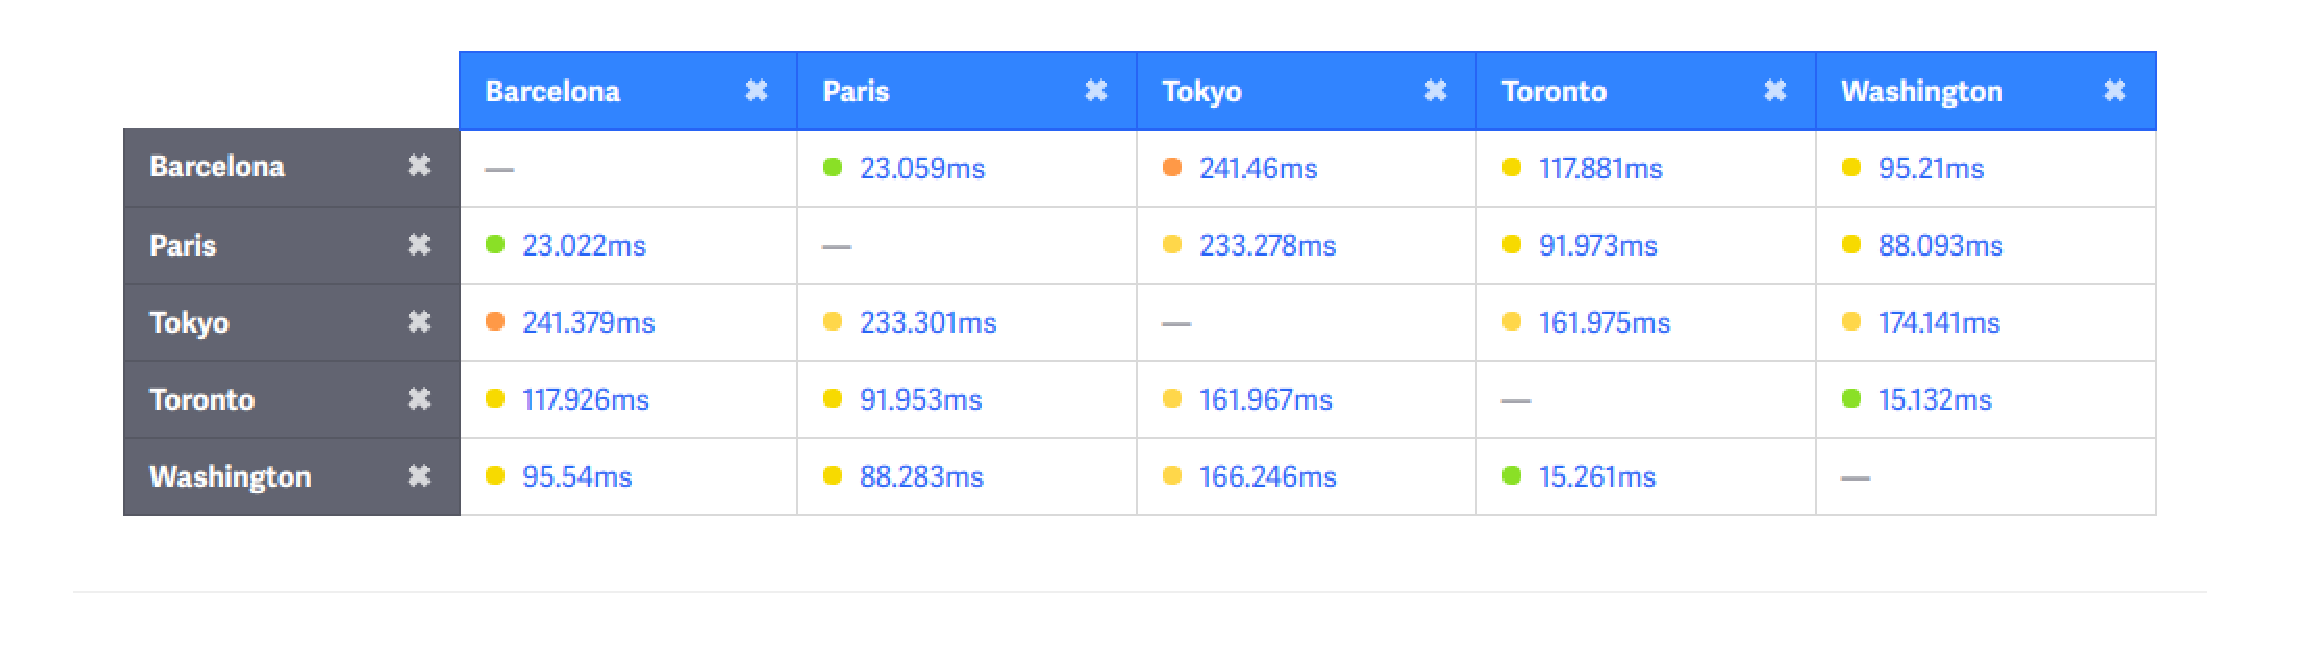
\includegraphics[width=160mm]{pht/Screenshot.eps}
  \end{center}
	\caption{参照したping値\cite{pings}}
  \label{fig:pings}
\end{figure*}
%
\ref{teian} 節の提案手法の実験を行う為に,実際に履歴交差法を行うことが
できるノードを実装した.実装するにあたり,文献\cite{hamatsu2018}を参考にした.
%今回は紙面の都合上,アルゴリズム1の実装と実験結果のみを紹介する.

以下に実装した通信プロトコルを示す.

\hspace{5mm}
%
\begin{enumerate}
\item \textbf{MSG\_REQUEST\_CROSS\_REFERENCE (MSG\_1)}\\
\hspace{12mm} (履歴交差の依頼 )
\item \textbf{MSG\_ACCEPT\_CROSS\_REFFERENCE (MSG\_2)}\\
\hspace{12mm}  (履歴交差依頼の承認 )
  \item \textbf{MSG\_START\_CROSS\_REFFERENCE (MSG\_3)}\\
\hspace{12mm}  (履歴交差の開始号令 )
  \item \textbf{MSG\_CROSS\_REFFERENCE (MSG\_4)}\\
\hspace{12mm}  (履歴交差を行いたいblock内容の共有 )
  \item \textbf{MSG\_COMPLETE\_CROSS\_REFERENCE (MSG\_5)} \\
\hspace{12mm}  (履歴交差の完了通知 )
\end{enumerate}
%
\hspace{5mm}

ローカル環境に構築した環境において実験を行った.
今回は簡単の為に,特定(ドメイン$D_2$)の中心コアノードが2分間隔で履歴交差の依頼を
他ドメインの中心コアノードに行い,履歴交差を開始させることとした.

\subsection{実装した履歴交差法の動作}
Phase1では,
ドメイン$D_2$の中心コアノードが履歴交差の依頼 (\textbf{MSG\_1})
を他ドメインの中心コアノードに送信し,ドメイン$D_2$以外の中心コアノードが受信する.
依頼を受信した各ドメインは履歴交差の依頼を了承する返信 (\textbf{MSG\_2})
をドメイン$D_2$に送信する.
ドメイン$D_2$の中心コアノードは,他の全てのドメインから了承の返信を受け取ったら,
履歴交差を開始する号令 (\textbf{MSG\_3}) を他ドメインの中心コアノード
に送信し,履歴交差を行いたい$l$-確定ブロックのデータを各ドメインの中心コアノードに
ブロードキャストする (\textbf{MSG\_4}).
同様に号令を受け取った$D_2$以外の中心コアノードは,各ドメインの中心コアノードにブロードキャスト
を行う.個々のドメインの中心コアノードは全てのドメインからの確定ブロックのデータを受取り,
データを暗号学的ハッシュ関数にかけてhash値にする.以上でPhase1は完了となる.

Phase2では,
Phase1の履歴交差部を書き込む為のマイングを行う.
本研究におけるマイニングは,ビットコンブロックチェーンにおけるPoWと同様のものである.
今回の実験では,PoWの難易度を5とした.
今回実験を行ったマシンでは,この難易度でブロックを生成するのに10秒程度の時間がかかっている.
履歴交差を行ったブロックが$l$-確定ブロックとなった時点でPhase2は完了となる.

最後にPhase3では,
マイニングを完了したブロックが,履歴交差を行ったブロックから$l$-確定ブロックとなった段階で,
他ドメインの中心コアノードに履歴交差に成功したことをブロードキャストする
 (\textbf{MSG\_5}).
今回の実験では,$l=3$とした.ブロードキャストを送信した時点でPhase 3は完了となる.

\subsection{通信遅延の考慮}
ドメインの最小規模の1国$2$〜$4$ドメイン程度で分割することを想定している.
従って,ドメイン間の通信は,他国間の通信の想定をする必要がある.
今回の実装には,多国間で通信遅延を考慮し通信遅延処理を追加し実装した.

\subsubsection{疑似通信遅延機能の実装}
各ドメインがBalcelona,Tokyo,Paris,Toronto,Washingtonにあるとし,履歴交差の依頼を行うドメイン$D_2$はTokyoのものとした.
2020年2月9日のpingのRTTにかかる時間\cite{pings}を参考にすることで,送信先のポート番号で送信先ドメインを区別して,
sleep関数を利用することで遅延を発生させた.

参考にした文献\cite{pings}は,unixコマンドラインツールのpingを用いており,ウインドウサイズを今回は$32$[Byte]とすると,
pingのRTTをP[ms]から,送信データサイズをB[Byte]に応じた通信遅延Lは,以下の式で表される.
\begin{equation}
  \label{byt}
    L = \frac{BP}{32} [sec]
\end{equation}
送信するデータサイズと送り先のポート番号に応じて通信遅延Lを発生させる処理とした.
通信する際におおよそ0.1〜2秒程度の通信遅延Lが発生している.
実際に参照した遅延時間を図\ref{fig:pings},算出したTokyoから150〜500[Byte]の疑似データサイズを
他のドメインへの送信した際の通信遅延Lの上限値を表\ref{Byte} に示す.

\begin{table}[H]%挿入図
  \centering
  \caption{Tokyoからの各ドメインへの疑似通信遅延(小数第2以下は省略)}
  \label{Byte}
  \begin{tabular}{c|c|c|c|c|}
  \cline{2-5}
  [sec]                       & Barcelona &    Paris   &   Toronto  & Washington \\ \hline
  \multicolumn{1}{|c|}{Tokyo} &  1.0〜3.8 &  1.0〜3.8  &  0.6〜2.4  &  0.8〜2.6  \\ \hline
  \end{tabular}
\end{table}

\subsection{t-故障耐性の実装}
本研究における故障は,フリーズ等の機器故障を故障状態として定義している.
履歴交差法を行う際にLayer0における各ドメインの中心コアノード以下の状態で故障することがある.

\begin{enumerate}
  \item 履歴交差の依頼を出し履歴交差法の号令を取る中心コアノードの故障(状態A)\\
  \hspace{12mm} 
  \item 履歴交差の依頼を受け,履歴交差に参加するノードの故障(状態B)\\
  \hspace{12mm} 
\end{enumerate}

履歴交差の依頼を出す中心コアノード(状態A)が故障してしまうと
履歴交差の依頼を出すノードが不在になり履歴交差法を実行ステップに移行できなくなる.
状態Aの統率役不在(故障)時を回避するために\ref{Raft}節のRaft Consensus Algorithm\ref{Raft}を用いる.

履歴交差の依頼を受け,履歴交差に参加するノードの故障(状態B)が,
故障してしまった場合はリーダー権を保持しているノードがタイムアウトで履歴交差から除外を行う.


\subsubsection{実験環境}
本研究における実験環境を以下の図\ref{fig:kankyou}に示す.
\begin{figure}[H]%挿入図
  \begin{center}
    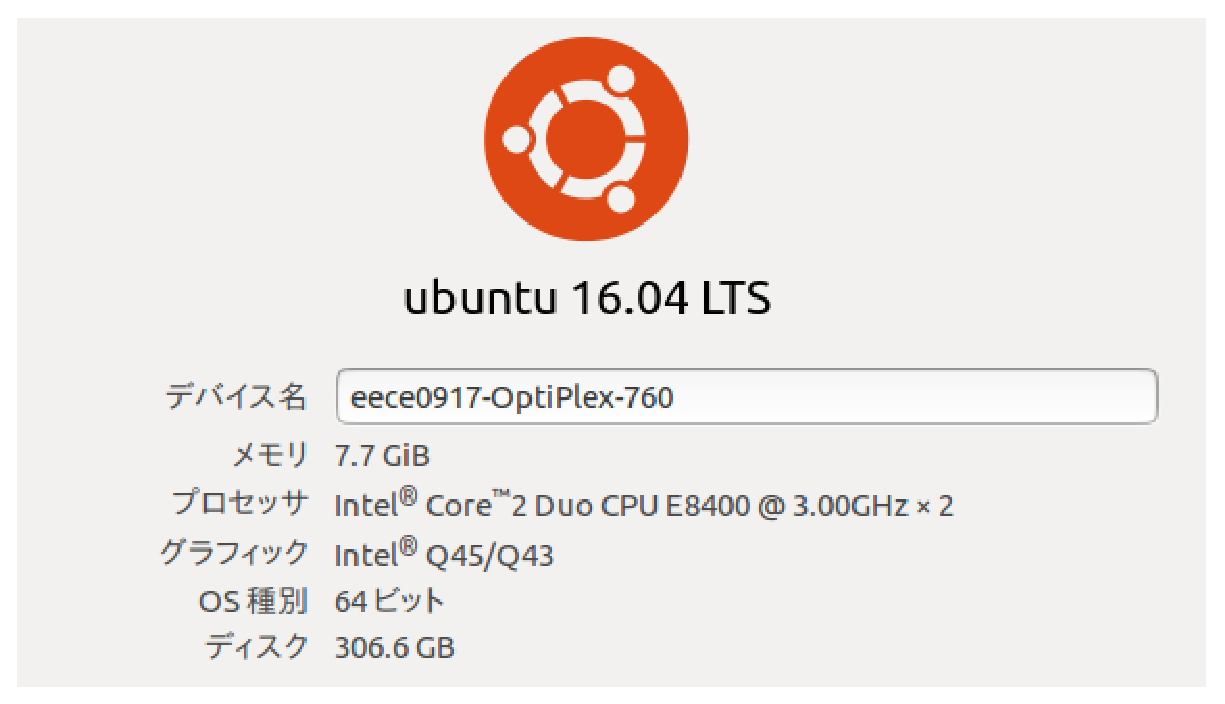
\includegraphics[width=100mm]{pht/kankyou.eps}
  \end{center}
  \caption{実験環境のシステム構成}
  \label{fig:kankyou}
\end{figure}
%
\begin{description}
  \item プロセッサ:$\text{Intel}^\text{\textregistered}$$\text{Core}^\text{TM}\text{2DUO CPU E8400@3.00GHz}\times2$
  \item メモリ:$8$GB
  \item OS:ubuntu16.04LTS
  \item 言語:Python3
\end{description}
以上の環境を用いて実験を行った.

\subsubsection{理論的性能評価}
%ここ

\subsubsection{実験結果}
\ref{}節で実装したプロトコルを用いて,履歴交差を1000回行い,各Phaseが終了するまでにかかる
遅延時間分布と履歴交差法の成功率について調査した.
前節で解説した通信プロトコルを用いて実験を行った結果として,各Phaseでの
遅延時間の分布を図\ref{fig:phase1}, \ref{fig:phase2}, \ref{fig:phase3}に示す.
%
\begin{figure}[H]%挿入図
  \begin{center}
    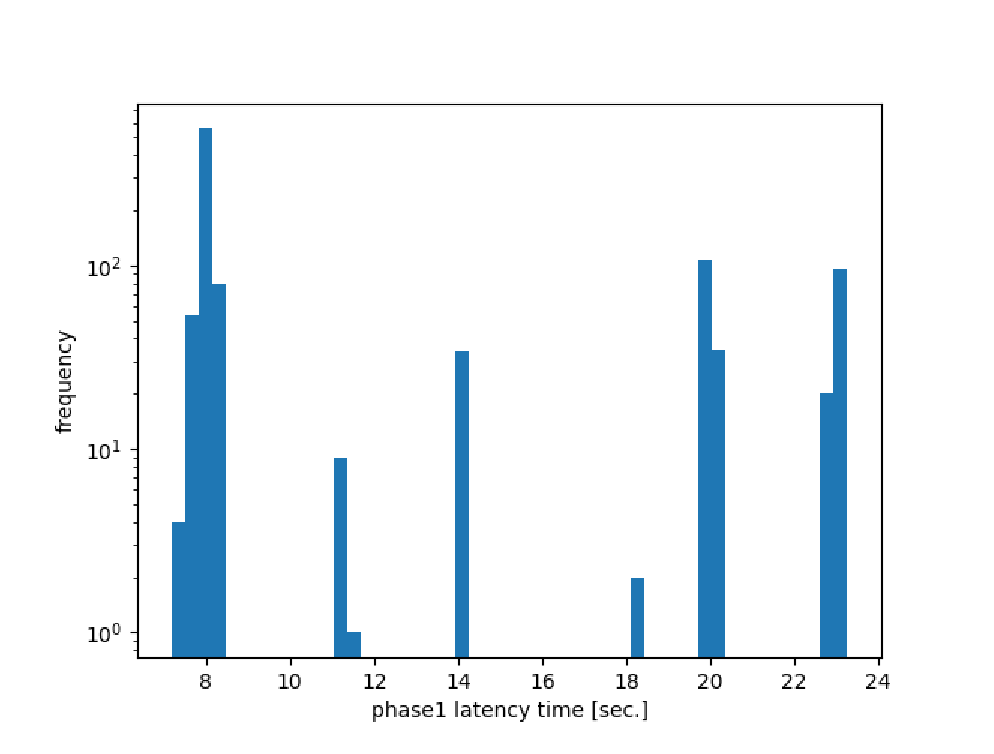
\includegraphics[width=100mm]{pht/phase1-sec-hist.eps}
  \end{center}
  \caption{Phase1の計測時間}
  \label{fig:phase1}
\end{figure}
%
%
\begin{figure}[H]%挿入図
  \begin{center}
    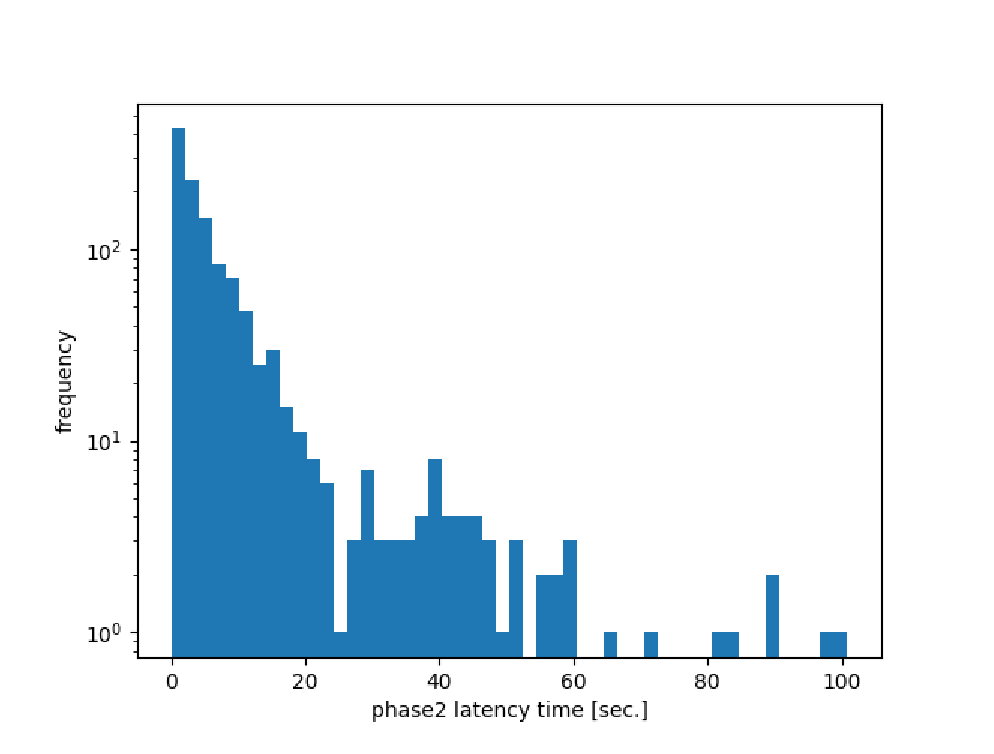
\includegraphics[width=100mm]{pht/phase2-sec-hist.eps}
  \end{center}
  \caption{Phase2の計測時間}
  \label{fig:phase2}
\end{figure}
%
%
\begin{figure}[H]%挿入図
  \begin{center}
    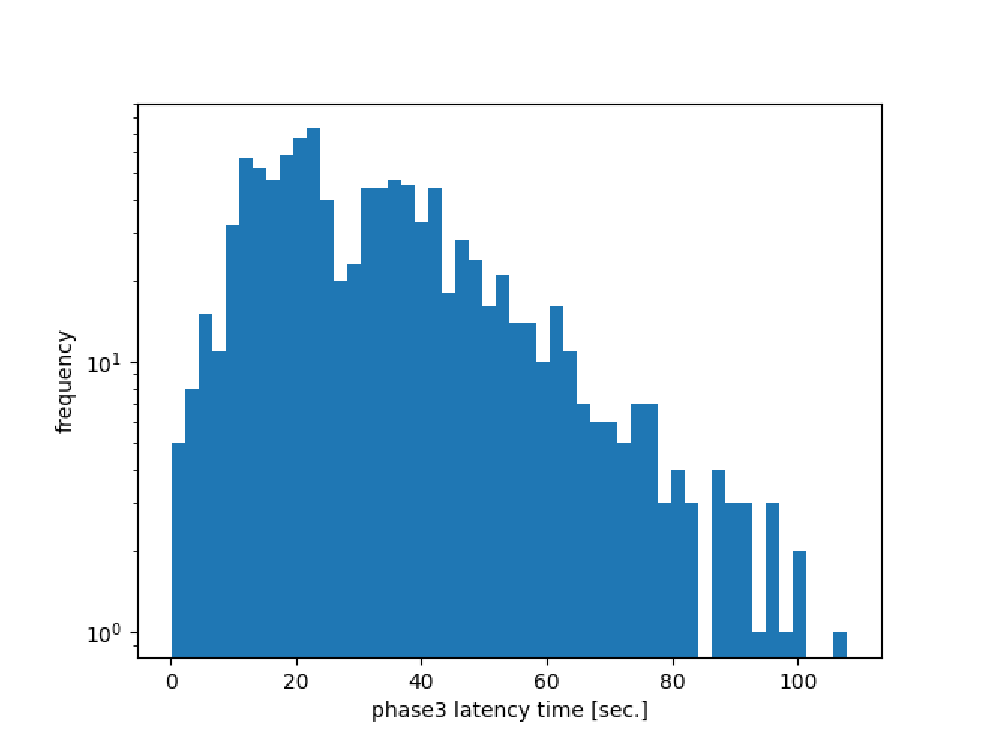
\includegraphics[width=100mm]{pht/phase3-sec-hist.eps}
  \end{center}
  \caption{Phase3の計測時間}
  \label{fig:phase3}
\end{figure}
%
Phase 1は殆どが8秒以下で終わっているが,場合によっては
最悪20秒程度かかることもあることが分かる.
Phase 2はマイニングを行うことから,指数分布に従っている
ことが分かる.
Phase 3は全てのノードのマイニングが完了するのを待つこと
から,タイミングが悪い場合は100秒程度待つ必要があることが分かる.
全てのPhaseを合計すると120秒程度になることから,履歴交差にかかる時間を見積もることができた.

また,1000回の履歴交差のうち,失敗は0回であった.従って,
成功率は100\%となった.

プロトコルを用いて,履歴交差を1000回行い,各Phaseが終了するまでにかかる
遅延時間分布と履歴交差法の成功率について調査した.
ここで,Layer 0である中心コアノードをドメイン$D_1, D_2, D_3, D_4, D_5$から
それぞれ1つの5ノードからなる状況を想定し,それらの間にP2Pネットワークを
ローカルに構築した環境において実験を行った.
今回は簡単の為に,特定(ドメイン$D_2$)の中心コアノードが2分間隔で履歴交差の依頼を
他ドメインの中心コアノードに行い,履歴交差を開始させることとした.

Phase1では,
ドメイン$D_2$の中心コアノードが履歴交差の依頼 (\textbf{MSG\_REQUEST\_CROSS\_REFERENCE})
を他ドメインの中心コアノードに送信し,ドメイン$D_2$以外の中心コアノードが受信する.
依頼を受信した各ドメインは履歴交差の依頼を了承する返信 (\textbf{MSG\_ACCEPT\_CROSS\_REFFERENCE})
をドメイン$D_2$に送信する.
ドメイン$D_2$の中心コアノードは,他の全てのドメインから了承の返信を受け取ったら,
履歴交差を開始する号令 (\textbf{MSG\_START\_CROSS\_REFFERENCE}) を他ドメインの中心コアノード
に送信し,履歴交差を行いたい$l$-確定ブロックのデータを各ドメインの中心コアノードに
ブロードキャストする (\textbf{MSG\_CROSS\_REFFERENCE}).
同様に号令を受け取った$D_2$以外の中心コアノードは,各ドメインの中心コアノードにブロードキャスト
を行う.個々のドメインの中心コアノードは全てのドメインからの確定ブロックのデータを受取り,
データを暗号学的ハッシュ関数にかけてhash値にする.以上でPhase1は完了となる.

Phase2では,
Phase1の履歴交差部を書き込む為のマイングを行う.今回の実験では,PoWの難易度を5とした.
今回実験を行ったマシンでは,この難易度でブロックを生成するのに10秒程度の時間がかかっている.
履歴交差を行ったブロックが$l$-確定ブロックとなった時点でPhase2は完了となる.

最後にPhase3では,
マイニングを完了したブロックが,履歴交差を行ったブロックから$l$-確定ブロックとなった段階で,
他ドメインの中心コアノードに履歴交差に成功したことをブロードキャストする
 (\textbf{MSG\_COMPLETE\_CROSS\_REFERENCE}).
今回の実験では,$l=3$とした.ブロードキャストを送信した時点でPhase 3は完了となる.
\newpage
%%----------------------------------------------------------------------
\section{結論}
%%----------------------------------------------------------------------
本研究では,独自のブロックチェーンを管理する複数のドメイン間で
定期的にブロックチェーンの状態を共有することで,互いのブロック
チェーンにヒステリシス署名を書き込み合う履歴交差法を提案した.

提案手法について理論的および実験的観点から,
改ざん耐性の向上比率について理論的に評価した.
一般にドメイン数が増加するほど,改ざん耐性向上比率$R$の分布の
ピークが大きい方にシフトすることが分かった.
また,ドメイン数が増えると分布の分散も大きくなることが確認できる.
スケールパラメータ$\alpha=2,3$の比較により,$\alpha$が小さくなる
ほど,改ざん耐性向上比率$R$の分布のピークが小さい方にシフトすることも分かった.

次に提案した履歴交差法を行うために以下の実装を行った.
\begin{enumerate}
  \item 履歴交差法を行うための通信プロトコルの設計・中心コアノードの実装\\
  \hspace{12mm}
  \item t-故障耐性法の検討・実装\\
  \hspace{12mm}
  \item Raft-Consensus-AlgorithmによるLayer0のリーダー選定法の提案・実装\\
  \hspace{12mm}
\end{enumerate}

実際に実装を行ったノードで,履歴交差法にかかる通信遅延時間を計測し,その成功率も実験的に評価した.
その結果,120秒程度待つことで履歴交差法の全Phaseが完了することが見積もれた.
また今回の実験特定の条件下ではあるが,履歴交差法の成功率は100\%となった.

またRaftのを用いたリーダーの選定の実装及び,t-故障耐性の実装も行った.

今後の課題としては,Raftのリーダーとして主張し続けるノード動作の考慮やドメイン分割の自律形成法の提案,
海外のレンタルサーバー間で実際の通信遅延発生状況下実験することや,
想定される様々な状況において安定して履歴交差法が行えるように実験を継続することがある.
また,理論的に得られた改ざん耐性向上比率を実験的に評価することがある.

\newpage
%%----------------------------------------------------------------------
\section*{謝辞}
%%----------------------------------------------------------------------

本研究は,令和2年度修士研究として,千葉工業大学大学院工学研究科電気電子情報工学専攻准教授 藤原明広先生のもとで行ったものである.
本研究を遂行するあたり,適切なご指導,御助言をして頂いた藤原明広先生に深く感謝の意を表する.
同専攻教授 菅原真司先生,並びに同専攻教授 枚田明彦先生には本論文を査読していただき,有益なご意見,コメントを頂いた.ここに感謝の意を表する.
また藤原研究室の各位には,研究遂行にあたり日頃より有益なご討論ご助言を戴いた.
この機会に皆様に深く感謝の意を表す.

\newpage
%%----------------------------------------------------------------------
%% 参考文献
%%----------------------------------------------------------------------

\begin{thebibliography}{99}
\bibitem{Bitcoin}
S.Nakamoto,
``Bitcoin: A Peer-to-Peer Electronic Cash System'' (2008).
\url {https://Bitcoin.org/Bitcoin.pdf} (2020年1月7日閲覧確認)

\bibitem{fujihara1}
A. Fujihara,
``Proposing a system for collaborative traffic information gathering 
and sharing incentiviz by blockchain technology,''
Advances in Intelligent Networking and Collaborative Systems,
pp.170-182, Springer (2019).

\bibitem{fujihara2}
A. Fujihara,
``PoWaP: Proof of Work at Proximity for a crowdsensing system for 
collaborative traffic information gathering,'' 
Internet of Things, 100046, Elsevier (2019).

\bibitem{suzaki}
洲崎誠一,松本勉,
電子署名アリバイ実現機構 -ヒステリシス署名と履歴交差-
情報処理学会論文誌,Vol.43, No.8, pp.2381-2393, (2002).

\bibitem{saito}
K. Saito,T. Kubo,"BBc-1: Beyond Blockchain One" (2018).
\url{https://beyond-blockchain.org/public/bbc1-design-paper.pdf} (2020年1月7日閲覧確認)

\bibitem{bloX}
bloXroute, \url{https://bloxroute.com} (2020年1月7日閲覧確認)

\bibitem{atomicswap}
Atomic swap, \url{https://en.Bitcoin.it/wiki/Atomic_swap#Algorithm}(2020年2月13日閲覧確認)

\bibitem{manabe}
真鍋義文, 「分散処理システム」森北出版 (2013).

\bibitem{hamatsu2018}
濱津誠, 「ゼロから創る暗号通貨」PEAKS出版 (2018).

\bibitem{pings}
WonderNetwork, \url{https://wondernetwork.com/pings}(2020年2月10日閲覧確認)

\bibitem{Raft Consensus Algorithm}


\end{thebibliography} 

%%----------------------------------------------------------------------
%\chapter{研究業績} % 研究業績
%%----------------------------------------------------------------------
%\AchieveItem{Hoge}
%ーーーーーーーーー.

%\AchieveItem{Hogeresults2}
%ーーーーーーーーー.

%\end{Achievements}


\newpage
\appendix
\def\thesection{付録}
\section{\\コード}

%\part{name}
%\begin{verbatim}
%  #include <iostream>
%  using namespace std;
%  int main() {
%  for(int i = 1; i <= 5; i++) {
%  cout << "こんにちは, C++ の世界! " << i << endl;
%  }
%  return 0;
%  }
%\end{verbatim}
%\verb|\usepackage{ascmac}|して\verb|screen| 環境を使うと,枠がつきます.

コードを載せる.

\newpage
\section{\\補足}

補足説明があればのせる.

\end{document}